\documentclass[a4paper, 12pt]{article}
%DIF LATEXDIFF DIFFERENCE FILE
%DIF DEL previous_version.tex                Fri Aug 19 09:43:01 2022
%DIF ADD tracking_selection_manuscript.tex   Thu Aug 25 13:44:13 2022

% basic package list
%\usepackage[T1]{fontenc}
\usepackage{fontspec}
\defaultfontfeatures{Mapping=tex-text}
\usepackage[margin=25mm]{geometry}
\usepackage{amsmath}
\usepackage{amsfonts}
\usepackage{amssymb}
\usepackage{graphicx}

% other packages
\usepackage{xunicode}
\usepackage{xltxtra}
\usepackage{hyperref}                       % hyperlinks
\usepackage{booktabs}                      % professional-quality tables
\usepackage{indentfirst}                     % to indent section first paragraph
\usepackage{url}                                 % simple URL typesetting
\usepackage{natbib}
\usepackage[modulo]{lineno}
\usepackage{sectsty}                          % to change section font size
\usepackage[flushleft]{threeparttable} % table with note
\usepackage[labelfont=bf]{caption}
\usepackage{lineno}
\usepackage{courier}

% black hypelinks with no border
\hypersetup{
    colorlinks,
    citecolor=black,
    filecolor=black,
    linkcolor=black,
    urlcolor=black
}

% set additional parameters
\setcitestyle{authoryear,open={(},close={)}}
\graphicspath {{Figures/}}

\sectionfont{\fontsize{14}{19}\selectfont}
\subsectionfont{\fontsize{12}{17}\selectfont}
\linenumbers

% reduce page number font size
\renewcommand*{\thepage}{\footnotesize\arabic{page}}

% Keywords command
\providecommand{\keywords}[1]
{
  \small	
  \textbf{\textit{Keywords---}} #1
}

%\newcommand{\beginsupplement}{%
%        \setcounter{table}{0}
%        \renewcommand{\thetable}{S\arabic{table}}%
%       \setcounter{figure}{0}
%        \renewcommand{\thefigure}{S\arabic{figure}}%
%     }

\title{Joint inference of adaptive and demographic history from temporal population genomic data}
\author{\small
            Vitor A. C. Pavinato$^{1,2,3}$, Stéphane De Mita$^4$, Jean-Michel Marin$^2$, Miguel de Navascués$^{1,5*}$}
\date{{\footnotesize % 
    $^1$CBGP, INRAE, CIRAD, IRD, Montpellier SupAgro, Université de Montpellier, Montpellier, France\\%
    $^2$UMR Institut Montpelliérain Alexander Grothendieck, Université de Montpellier, France \\%  
    $^3$Entomology Dept., CFAES, The Ohio State University, Wooster, USA\\%
    $^4$UMR Interactions Arbres-Microorganismes, INRAE, France \\%
    $^5$Human Evolution, Department of Organismal Biology, Uppsala University, Uppsala, Sweden\\%  
    $^*$corresponding author: miguel.navascues@inrae.fr\\[2ex]%
    }
    \footnotesize\today    
}
%DIF PREAMBLE EXTENSION ADDED BY LATEXDIFF
%DIF UNDERLINE PREAMBLE %DIF PREAMBLE
\RequirePackage[normalem]{ulem} %DIF PREAMBLE
\RequirePackage{color}\definecolor{RED}{rgb}{1,0,0}\definecolor{BLUE}{rgb}{0,0,1} %DIF PREAMBLE
\providecommand{\DIFaddtex}[1]{{\protect\color{blue}\uwave{#1}}} %DIF PREAMBLE
\providecommand{\DIFdeltex}[1]{{\protect\color{red}\sout{#1}}}                      %DIF PREAMBLE
%DIF SAFE PREAMBLE %DIF PREAMBLE
\providecommand{\DIFaddbegin}{} %DIF PREAMBLE
\providecommand{\DIFaddend}{} %DIF PREAMBLE
\providecommand{\DIFdelbegin}{} %DIF PREAMBLE
\providecommand{\DIFdelend}{} %DIF PREAMBLE
\providecommand{\DIFmodbegin}{} %DIF PREAMBLE
\providecommand{\DIFmodend}{} %DIF PREAMBLE
%DIF FLOATSAFE PREAMBLE %DIF PREAMBLE
\providecommand{\DIFaddFL}[1]{\DIFadd{#1}} %DIF PREAMBLE
\providecommand{\DIFdelFL}[1]{\DIFdel{#1}} %DIF PREAMBLE
\providecommand{\DIFaddbeginFL}{} %DIF PREAMBLE
\providecommand{\DIFaddendFL}{} %DIF PREAMBLE
\providecommand{\DIFdelbeginFL}{} %DIF PREAMBLE
\providecommand{\DIFdelendFL}{} %DIF PREAMBLE
%DIF HYPERREF PREAMBLE %DIF PREAMBLE
\providecommand{\DIFadd}[1]{\texorpdfstring{\DIFaddtex{#1}}{#1}} %DIF PREAMBLE
\providecommand{\DIFdel}[1]{\texorpdfstring{\DIFdeltex{#1}}{}} %DIF PREAMBLE
\newcommand{\DIFscaledelfig}{0.5}
%DIF HIGHLIGHTGRAPHICS PREAMBLE %DIF PREAMBLE
\RequirePackage{settobox} %DIF PREAMBLE
\RequirePackage{letltxmacro} %DIF PREAMBLE
\newsavebox{\DIFdelgraphicsbox} %DIF PREAMBLE
\newlength{\DIFdelgraphicswidth} %DIF PREAMBLE
\newlength{\DIFdelgraphicsheight} %DIF PREAMBLE
% store original definition of \includegraphics %DIF PREAMBLE
\LetLtxMacro{\DIFOincludegraphics}{\includegraphics} %DIF PREAMBLE
\newcommand{\DIFaddincludegraphics}[2][]{{\color{blue}\fbox{\DIFOincludegraphics[#1]{#2}}}} %DIF PREAMBLE
\newcommand{\DIFdelincludegraphics}[2][]{% %DIF PREAMBLE
\sbox{\DIFdelgraphicsbox}{\DIFOincludegraphics[#1]{#2}}% %DIF PREAMBLE
\settoboxwidth{\DIFdelgraphicswidth}{\DIFdelgraphicsbox} %DIF PREAMBLE
\settoboxtotalheight{\DIFdelgraphicsheight}{\DIFdelgraphicsbox} %DIF PREAMBLE
\scalebox{\DIFscaledelfig}{% %DIF PREAMBLE
\parbox[b]{\DIFdelgraphicswidth}{\usebox{\DIFdelgraphicsbox}\\[-\baselineskip] \rule{\DIFdelgraphicswidth}{0em}}\llap{\resizebox{\DIFdelgraphicswidth}{\DIFdelgraphicsheight}{% %DIF PREAMBLE
\setlength{\unitlength}{\DIFdelgraphicswidth}% %DIF PREAMBLE
\begin{picture}(1,1)% %DIF PREAMBLE
\thicklines\linethickness{2pt} %DIF PREAMBLE
{\color[rgb]{1,0,0}\put(0,0){\framebox(1,1){}}}% %DIF PREAMBLE
{\color[rgb]{1,0,0}\put(0,0){\line( 1,1){1}}}% %DIF PREAMBLE
{\color[rgb]{1,0,0}\put(0,1){\line(1,-1){1}}}% %DIF PREAMBLE
\end{picture}% %DIF PREAMBLE
}\hspace*{3pt}}} %DIF PREAMBLE
} %DIF PREAMBLE
\LetLtxMacro{\DIFOaddbegin}{\DIFaddbegin} %DIF PREAMBLE
\LetLtxMacro{\DIFOaddend}{\DIFaddend} %DIF PREAMBLE
\LetLtxMacro{\DIFOdelbegin}{\DIFdelbegin} %DIF PREAMBLE
\LetLtxMacro{\DIFOdelend}{\DIFdelend} %DIF PREAMBLE
\DeclareRobustCommand{\DIFaddbegin}{\DIFOaddbegin \let\includegraphics\DIFaddincludegraphics} %DIF PREAMBLE
\DeclareRobustCommand{\DIFaddend}{\DIFOaddend \let\includegraphics\DIFOincludegraphics} %DIF PREAMBLE
\DeclareRobustCommand{\DIFdelbegin}{\DIFOdelbegin \let\includegraphics\DIFdelincludegraphics} %DIF PREAMBLE
\DeclareRobustCommand{\DIFdelend}{\DIFOaddend \let\includegraphics\DIFOincludegraphics} %DIF PREAMBLE
\LetLtxMacro{\DIFOaddbeginFL}{\DIFaddbeginFL} %DIF PREAMBLE
\LetLtxMacro{\DIFOaddendFL}{\DIFaddendFL} %DIF PREAMBLE
\LetLtxMacro{\DIFOdelbeginFL}{\DIFdelbeginFL} %DIF PREAMBLE
\LetLtxMacro{\DIFOdelendFL}{\DIFdelendFL} %DIF PREAMBLE
\DeclareRobustCommand{\DIFaddbeginFL}{\DIFOaddbeginFL \let\includegraphics\DIFaddincludegraphics} %DIF PREAMBLE
\DeclareRobustCommand{\DIFaddendFL}{\DIFOaddendFL \let\includegraphics\DIFOincludegraphics} %DIF PREAMBLE
\DeclareRobustCommand{\DIFdelbeginFL}{\DIFOdelbeginFL \let\includegraphics\DIFdelincludegraphics} %DIF PREAMBLE
\DeclareRobustCommand{\DIFdelendFL}{\DIFOaddendFL \let\includegraphics\DIFOincludegraphics} %DIF PREAMBLE
%DIF LISTINGS PREAMBLE %DIF PREAMBLE
\RequirePackage{listings} %DIF PREAMBLE
\RequirePackage{color} %DIF PREAMBLE
\lstdefinelanguage{DIFcode}{ %DIF PREAMBLE
%DIF DIFCODE_UNDERLINE %DIF PREAMBLE
  moredelim=[il][\color{red}\sout]{\%DIF\ <\ }, %DIF PREAMBLE
  moredelim=[il][\color{blue}\uwave]{\%DIF\ >\ } %DIF PREAMBLE
} %DIF PREAMBLE
\lstdefinestyle{DIFverbatimstyle}{ %DIF PREAMBLE
	language=DIFcode, %DIF PREAMBLE
	basicstyle=\ttfamily, %DIF PREAMBLE
	columns=fullflexible, %DIF PREAMBLE
	keepspaces=true %DIF PREAMBLE
} %DIF PREAMBLE
\lstnewenvironment{DIFverbatim}{\lstset{style=DIFverbatimstyle}}{} %DIF PREAMBLE
\lstnewenvironment{DIFverbatim*}{\lstset{style=DIFverbatimstyle,showspaces=true}}{} %DIF PREAMBLE
%DIF END PREAMBLE EXTENSION ADDED BY LATEXDIFF

\begin{document}
\maketitle

\begin{abstract}
Disentangling the effects of selection and drift is a long-standing problem in population genetics. Recently, simulations \DIFdelbegin \DIFdel{shows }\DIFdelend \DIFaddbegin \DIFadd{show }\DIFaddend that pervasive selection may bias the inference of demography. Ideally, models for the inference of demography and selection should account for the interaction between these two forces.
With simulation-based likelihood-free methods such as Approximate Bayesian Computation \DIFaddbegin \DIFadd{(ABC)}\DIFaddend , demography and selection parameters can be jointly estimated\DIFdelbegin \DIFdel{(ABC)}\DIFdelend . We propose \DIFdelbegin \DIFdel{a }\DIFdelend \DIFaddbegin \DIFadd{to use the }\DIFaddend ABC-Random Forests framework to \DIFdelbegin \DIFdel{jointly infer demographic }\DIFdelend \DIFaddbegin \DIFadd{infer demographic jointly }\DIFaddend and selection parameters from temporal population genomic data (e.g.\DIFaddbegin \DIFadd{, }\DIFaddend \ experimental evolution, monitored populations, ancient DNA). Our framework allowed the separation of demography (census size, $N$) from the genetic drift (effective population size, $N_{\mathrm{e}}$) \DIFdelbegin \DIFdel{, }\DIFdelend and the estimation of genome-wide parameters of selection. Selection parameters informed us about the adaptive potential of a population (the scale mutation rate of beneficial mutations, $\theta_{\mathrm{b}}$), the realized \DIFdelbegin \DIFdel{potential}\DIFdelend \DIFaddbegin \DIFadd{adaptation}\DIFaddend , as the number of strong beneficial under selection, and \DIFdelbegin \DIFdel{fitness diversity as the population }\DIFdelend \DIFaddbegin \DIFadd{population fitness as the }\DIFaddend genetic load. We applied this approach to a dataset of feral populations of honey bees (\textit{Apis mellifera}) collected in California, and we estimated parameters consistent with the biology and the recent history of this species.
\end{abstract}\hspace{12pt}

% keywords can be removed
\keywords{Temporal data, Population genomics, Machine learning, Adaptation}

\newpage

\section*{Introduction}

One aim of population genomics is to understand how demography and natural selection shape the genetic diversity of populations. A classical approach \DIFdelbegin \DIFdel{is to assume }\DIFdelend \DIFaddbegin \DIFadd{assumes }\DIFaddend that demography (migration, population subdivision, population size changes) leaves a genome-wide signal\DIFdelbegin \DIFdel{, whereas }\DIFdelend \DIFaddbegin \DIFadd{. In contrast, }\DIFaddend selection leaves a \DIFdelbegin \DIFdel{localizes }\DIFdelend \DIFaddbegin \DIFadd{localized }\DIFaddend signal close to where the causal mutation is located. Many methods follow this approach to infer demography or selection \citep[reviewed by][]{Beichman:2018bx, Casillas:2017jv}. \DIFdelbegin \DIFdel{Methods for demographic inference assume }\DIFdelend \DIFaddbegin \DIFadd{Demographic inference assumes }\DIFaddend that most of the genome evolves without the influence of selection and that any deviation from the mutation-drift equilibrium observed in the data was caused by demographic events \citep{Beichman:2018bx}. \DIFdelbegin \DIFdel{For selection, the majority }\DIFdelend \DIFaddbegin \DIFadd{Many }\DIFaddend of the methods search for locus-specific signals \DIFdelbegin \DIFdel{left by the beneficial mutation }\DIFdelend \DIFaddbegin \DIFadd{of selection left }\DIFaddend on nearby neutral mutations \citep{Tajima:1989un, Fay:2000dl, Kim:2004ih} (low genetic diversity and high differentiation) to localize the \DIFdelbegin \DIFdel{beneficial }\DIFdelend \DIFaddbegin \DIFadd{region affected by selection }\DIFaddend mutation, assuming \DIFdelbegin \DIFdel{constant population size \mbox{%DIFAUXCMD
\citep{Nielsen:2005kx, Pool:2010eh}}\hspace{0pt}%DIFAUXCMD
}\DIFdelend \DIFaddbegin \DIFadd{a specific demography \mbox{%DIFAUXCMD
\citep[constant population size in early methods;][]{Nielsen:2005kx, Pool:2010eh}}\hspace{0pt}%DIFAUXCMD
}\DIFaddend .

Conducting demographic and selection inference separately may have some shortcomings. First, there is the assumption that the signal left by demography is little affected by selection because \DIFaddbegin \DIFadd{the }\DIFaddend selection is rare. However, linked selection can affect neutral and weakly selected sites that are far from the mutation targeted by selection \citep{Sella:2009hs, Neher:2013ju} and selection can be pervasive \citep{Sella:2009hs, Lange:2018fl}. In addition, some methods for selection scans are not robust to misspecifications of demographic history. Consequently, an unspecified bottleneck or population increase, for example, can inflate the \DIFdelbegin \DIFdel{type I error }\DIFdelend \DIFaddbegin \DIFadd{false positive }\DIFaddend rate of genome scans \citep{Jensen:2005ky, Jensen:2007jw, Schrider:2016gg}. These findings highlight the necessity of inferential methods that jointly accounts for the multiple evolutionary forces that act on populations \citep{Lin:2011jv, Li:2012bh, Bank:2014hx}. 

It is \DIFdelbegin \DIFdel{difficult to obtain }\DIFdelend \DIFaddbegin \DIFadd{often difficult to calculate }\DIFaddend the likelihood of models including demography and selection \citep[but see][]{Vitalis:2014ja}. Methods that rely on simulations provide \DIFdelbegin \DIFdel{alternatives to the use of }\DIFdelend \DIFaddbegin \DIFadd{easier alternatives to using }\DIFaddend likelihood functions \citep{Csillery:2010jd, Schrider:2018ei}. One of the first works that proposed such \DIFaddbegin \DIFadd{a }\DIFaddend strategy addressed the inference of local adaptation \citep{Bazin:2010dv}. With coalescent simulations of an island model, \citet{Bazin:2010dv} estimated demographic parameters and inferred the number of loci under selection. In their simulations, \DIFaddbegin \DIFadd{the }\DIFaddend selection was modeled as \DIFdelbegin \DIFdel{differential }\DIFdelend locus-specific migration rates in which a selected locus had lower migration rates than \DIFdelbegin \DIFdel{neutrally-evolved }\DIFdelend \DIFaddbegin \DIFadd{neutral }\DIFaddend loci. However, locus-specific migration rates or effective population size \citep[as in][]{Roux:2016gm, Fraisse:2021gg} represent \DIFaddbegin \DIFadd{crude }\DIFaddend approximations of the selection process. Forward-in-time simulation allows more realistic models of selection. These were used to make inferences on $N_\mathrm{e}$ in the presence of selection by \citet{Sheehan:2016caa} (\DIFdelbegin \DIFdel{for selective sweep }\DIFdelend \DIFaddbegin \DIFadd{selective sweeps }\DIFaddend and balancing selection) and \citet{Johri:2020ee} (background selection). However, these works rely on simulations of few independent loci-not more than 50Kbp-which prevents the \DIFdelbegin \DIFdel{modelling }\DIFdelend \DIFaddbegin \DIFadd{modeling }\DIFaddend of genome-wide effects of selection as the reduction of effective population size due to the variance of reproductive success of individuals \DIFdelbegin \DIFdel{\mbox{%DIFAUXCMD
\citep[e.g.][]{Santiago:1995wx}}\hspace{0pt}%DIFAUXCMD
}\DIFdelend \DIFaddbegin \DIFadd{\mbox{%DIFAUXCMD
\citep{Santiago:1995wx} }\hspace{0pt}%DIFAUXCMD
or the combined effects of mutations on individual fitness}\DIFaddend .
Nevertheless, this strategy brought new insights into the dynamics of selection. \DIFdelbegin \DIFdel{For instance, }\DIFdelend \citet{Laval:2019jo} estimated the number of past selective sweeps \DIFdelbegin \DIFdel{that occurred }\DIFdelend in the human genome in the past \DIFdelbegin \DIFdel{10}\DIFdelend \DIFaddbegin \DIFadd{100}\DIFaddend ,000 \DIFaddbegin \DIFadd{years}\DIFaddend , their intensity, and their age. Besides some limitations, these works exemplify the power of likelihood-free methods \DIFdelbegin \DIFdel{for the inference of }\DIFdelend \DIFaddbegin \DIFadd{to infer }\DIFaddend the complex interaction between demography and selection.

Most population genetic studies use samples collected at \DIFdelbegin \DIFdel{one time }\DIFdelend \DIFaddbegin \DIFadd{a one-time }\DIFaddend point to infer the neutral processes (mutation, recombination, random genetic drift) and selection throughout the history of populations. Temporal data allows a better understanding of recent evolutionary processes \DIFdelbegin \DIFdel{\mbox{%DIFAUXCMD
\citep{Feder:2021bt, Dehasque:2020ku} }\hspace{0pt}%DIFAUXCMD
}\DIFdelend \DIFaddbegin \DIFadd{\mbox{%DIFAUXCMD
\citep[e.g.][]{Feder:2021bt, Dehasque:2020ku} }\hspace{0pt}%DIFAUXCMD
}\DIFaddend because they contain information about the allele frequency changes through time. By tracking the allele frequency changes over time, it is possible to estimate the relative role of selection and drift. Consequently, temporal data has the potential to give us a better understanding of the interaction between drift and selection \citep[see for example,][]{Buffalo:2019ab, Buffalo:2020hq}. 

Here, we propose \DIFdelbegin \DIFdel{the use of ABC to jointly }\DIFdelend \DIFaddbegin \DIFadd{using ABC to }\DIFaddend estimate demography and positive selection from temporal genomic data \DIFaddbegin \DIFadd{jointly}\DIFaddend . In our framework, we use \DIFdelbegin \DIFdel{agent-based}\DIFdelend \DIFaddbegin \DIFadd{individual-based}\DIFaddend , forward-in-time simulations\DIFdelbegin \DIFdel{which allowed the modelling }\DIFdelend \DIFaddbegin \DIFadd{, which allow the modeling }\DIFaddend of the genome-wide\DIFdelbegin \DIFdel{and linked selection }\DIFdelend \DIFaddbegin \DIFadd{, linked selection and additive }\DIFaddend effects of beneficial mutations. Until recently, \DIFdelbegin \DIFdel{the use of }\DIFdelend such computationally demanding simulations in ABC inference \DIFdelbegin \DIFdel{was unrealistic since a great number of }\DIFdelend \DIFaddbegin \DIFadd{were unrealistic since many }\DIFaddend simulations are required to achieve accuracy in ABC \citep{Frazier:2018kq}. However, with the introduction of Random Forests (ABC-RF), it was possible to reduce the computational burden as fewer simulations are required to achieve reliable estimates \citep{Pudlo:2016il, Raynal:2019jj}. While many methods focus on the detection of targets of selection, our work addresses the inference of parameters that characterizes the genome-wide signal of demography and selection. Our genome-wide estimates \DIFdelbegin \DIFdel{showed to be }\DIFdelend \DIFaddbegin \DIFadd{were }\DIFaddend reasonably accurate for a wide \DIFdelbegin \DIFdel{rate of adaptation }\DIFdelend \DIFaddbegin \DIFadd{range of adaptation rates }\DIFaddend and strength of selection. We were able to separate the estimates of $N_{\mathrm{e}}$ \DIFdelbegin \DIFdel{, which reflect the short-term drift}\DIFdelend \DIFaddbegin \DIFadd{(a measure of genetic drift) }\DIFaddend from the population census size $N$. We also estimated the \DIFdelbegin \DIFdel{rate of }\DIFdelend influx of new beneficial mutations as measured by \DIFdelbegin \DIFdel{genome-wide }\DIFdelend \DIFaddbegin \DIFadd{the population }\DIFaddend scaled mutation rate of beneficial mutations. The separation between demography and drift \DIFdelbegin \DIFdel{, }\DIFdelend and the inference of genome-wide selection \DIFdelbegin \DIFdel{were only possible with the use of }\DIFdelend \DIFaddbegin \DIFadd{was only possible using }\DIFaddend latent variables. Latent variables emerged as properties of each simulation\DIFaddbegin \DIFadd{, }\DIFaddend and consequently, they better captured the emerging interaction between demography and selection than model parameters. We first evaluated the performance of an ABC-RF approach with forward-in-time simulations\DIFdelbegin \DIFdel{, and finally}\DIFdelend \DIFaddbegin \DIFadd{. Finally}\DIFaddend , we applied this framework to the analysis of a real time-series population genomics dataset of the feral population of honey bees (\textit{Apis mellifera}) \citep{Cridland:2018fx}. Our results were consistent with the \DIFdelbegin \DIFdel{biology of the species}\DIFdelend \DIFaddbegin \DIFadd{species' biology }\DIFaddend and with events that occurred recently in the history of the analyzed populations, taking into account the limitations of \DIFaddbegin \DIFadd{the current implementation of }\DIFaddend our approach.

\section*{Methods}

\subsection*{Inference model}

We assumed a closed population (no migration) of $N$ diploid individuals that evolved under a Wright-Fisher model with selection. \DIFdelbegin \DIFdel{Selection }\DIFdelend \DIFaddbegin \DIFadd{The population census size $N$ was constant, and selection }\DIFaddend only acted on \textit{de novo} beneficial mutations \DIFdelbegin \DIFdel{and }\DIFdelend that were allowed to arise in the population since the first generation \DIFaddbegin \DIFadd{(generation one corresponds to the first burn-in generation)}\DIFaddend . Every beneficial mutation had a selection coefficient of $s$ higher than zero\DIFaddbegin \DIFadd{, }\DIFaddend and all were co-dominant. The values of the selection coefficients $s$ were drawn from a gamma distribution with mean $\gamma$ \DIFdelbegin \DIFdel{. }\DIFdelend \DIFaddbegin \DIFadd{and scale equal parameter equals 1. }\DIFaddend Beneficial mutations entered the population with a rate of $\mu_\mathrm{b}$ per generation \DIFdelbegin \DIFdel{that is }\DIFdelend independent of the mutation selective strength. \DIFdelbegin \DIFdel{Consequetly }\DIFdelend \DIFaddbegin \DIFadd{Consequently, }\DIFaddend we defined the scaled mutation rate of the beneficial mutations per generation $\theta_\mathrm{b}$ as the product the population size $N$, the mutation rate of beneficial mutation $\mu_\mathrm{b}$ and the genome size $G$, $\theta_\mathrm{b} = 4N\mu_\mathrm{b}G$. This rate determines the amount of new beneficial mutations that \DIFdelbegin \DIFdel{arises }\DIFdelend \DIFaddbegin \DIFadd{arise }\DIFaddend in the population every generation. It can also be viewed as the waiting time for the appearance of a new beneficial mutation in the population. Populations with high $\theta_\mathrm{b}$ receive new beneficial mutations every generation \citep{Karasov:2010di}, but \DIFaddbegin \DIFadd{a }\DIFaddend population with low $\theta_\mathrm{b}$ needs to wait more time for a new beneficial mutation to arise.

We \DIFdelbegin \DIFdel{needed to divide the model in }\DIFdelend \DIFaddbegin \DIFadd{divided the model into }\DIFaddend two periods: 1) the burn-in period, \DIFdelbegin \DIFdel{that }\DIFdelend \DIFaddbegin \DIFadd{which }\DIFaddend is necessary to remove \DIFdelbegin \DIFdel{, }\DIFdelend from the simulations \DIFdelbegin \DIFdel{, }\DIFdelend any footprint of the initial \DIFdelbegin \DIFdel{parameters set}\DIFdelend \DIFaddbegin \DIFadd{simulation state}\DIFaddend ; the duration of this period was defined as the time necessary to contain all most recent common ancestors (MRCA) for all genomic regions in the simulation \DIFaddbegin \DIFadd{(}\textit{\DIFadd{i.e.}}\DIFadd{\ the burn-in was run until this condition was fulfilled)}\DIFaddend ; and 2) the inference period, where we defined the longitudinal samples of individuals; the sampled genotypes were used to make inference of demography and selection. \DIFdelbegin \DIFdel{This }\DIFdelend \DIFaddbegin \DIFadd{These }\DIFaddend two periods were defined by their time \DIFdelbegin \DIFdel{span and by }\DIFdelend \DIFaddbegin \DIFadd{spam and }\DIFaddend the population census size\DIFdelbegin \DIFdel{with }\DIFdelend \DIFaddbegin \DIFadd{, being }\DIFaddend $N_\mathrm{0}$ and $N$ as the \DIFdelbegin \DIFdel{sample }\DIFdelend \DIFaddbegin \DIFadd{population }\DIFaddend size of the burn-in and the inference period\DIFaddbegin \DIFadd{, respectively. Population size is constant within each simulated period and changes between periods}\DIFaddend .

\DIFdelbegin \DIFdel{The first }\DIFdelend \DIFaddbegin \DIFadd{First }\DIFaddend sample of individuals was taken at $t_1$, \DIFdelbegin \DIFdel{that was the first generation after }\DIFdelend the \DIFaddbegin \DIFadd{immediate next generation after }\DIFaddend burn-in \DIFdelbegin \DIFdel{period ended, and }\DIFdelend \DIFaddbegin \DIFadd{ended; }\DIFaddend the second was taken at $t_2$, after $\tau$ generations from $t_1$. Individuals were sampled following the sample plan II of \citet{Nei:1981vb}, where individuals were taken before \DIFdelbegin \DIFdel{their }\DIFdelend reproduction and permanently removed from the population. In this way\DIFaddbegin \DIFadd{, }\DIFaddend their genotypes did not contribute to the next generation\DIFdelbegin \DIFdel{genotypes}\DIFdelend .

Each \DIFdelbegin \DIFdel{individuals }\DIFdelend \DIFaddbegin \DIFadd{individual's }\DIFaddend genome of size $G$ (in base pairs) consisted of a single linkage group with \DIFaddbegin \DIFadd{a }\DIFaddend per base recombination rate per generation of \DIFdelbegin \DIFdel{$c_\mathrm{0}$. In this genome, we modeled the act of selection }\DIFdelend \DIFaddbegin \DIFadd{$r$. We modeled the selection effect in this genome }\DIFaddend by dividing it \DIFdelbegin \DIFdel{in }\DIFdelend \DIFaddbegin \DIFadd{into }\DIFaddend ``neutral'' and ``non-neutral'' regions. Non-neutral regions held both neutral and beneficial mutations. This division can be interpreted as a genomic architecture in which \DIFdelbegin \DIFdel{there are genic regions that }\DIFdelend \DIFaddbegin \DIFadd{genic regions }\DIFaddend have a combination of neutral (synonymous intron mutations) and selected (non-synonymous mutation) sites \DIFdelbegin \DIFdel{, and }\DIFdelend \DIFaddbegin \DIFadd{with }\DIFaddend intergenic regions (neutral mutations) \DIFdelbegin \DIFdel{but also other characteristics of the genome that would make the action of selection heterogeneous }\DIFdelend \DIFaddbegin \DIFadd{in between. However, this architecture allowed simulating the heterogeneous selection action }\DIFaddend along the genome. 
\DIFaddbegin 

\DIFaddend We chose this simplification because it is \DIFdelbegin \DIFdel{general and it was a }\DIFdelend \DIFaddbegin \DIFadd{a general and }\DIFaddend straightforward way to define independent priors for the relative number of non-neutral to neutral regions \DIFdelbegin \DIFdel{, }\DIFdelend and for the number of beneficial mutations in non-neutral regions. The probability of beneficial mutation to arise in the simulation \DIFdelbegin \DIFdel{, or their }\DIFdelend \DIFaddbegin \DIFadd{(}\textit{\DIFadd{i.e.}}\DIFadd{~the }\DIFaddend mutation rate per generation\DIFdelbegin \DIFdel{$\mu_\mathrm{b}$, }\DIFdelend \DIFaddbegin \DIFadd{, $\mu_\mathrm{b}$) }\DIFaddend was determined by the product of the proportion of non-neutral regions $P_\mathrm{R}$, the proportion of beneficial mutation in a non-neutral region $P_\mathrm{B}$ and the mutation rate per generation $\mu$. Figure~\ref{fig:model} shows a schematic representation of the model template (and see Table~S1 for a summary of the notation).

\begin{figure}[ht]
 \centering
 \DIFdelbeginFL %DIFDELCMD < \includegraphics[width=0.95\textwidth]{Figures/main_text/Figure1_model.pdf}
%DIFDELCMD <   %%%
\DIFdelendFL \DIFaddbeginFL \includegraphics[width=0.95\textwidth]{Figures/Figure1_model.pdf}
 \DIFaddendFL \small\caption{\textbf{A schematic representation of the model used to simulate temporal population genomic data.} (A) the population model \DIFdelbeginFL \DIFdelFL{that }\DIFdelendFL consisted of \DIFdelbeginFL \DIFdelFL{: }\DIFdelendFL 1) the burn-in period, where the number of generations was determined by the time necessary to contain the MRCA for all genomic regions. 2) the \DIFdelbeginFL \DIFdelFL{sampling }\DIFdelendFL \DIFaddbeginFL \DIFaddFL{inference }\DIFaddendFL period between the \DIFdelbeginFL \DIFdelFL{two time }\DIFdelendFL \DIFaddbeginFL \DIFaddFL{two-time }\DIFaddendFL points, where the inference of demography and selection was made. (B) the genomic architecture model \DIFdelbeginFL \DIFdelFL{that }\DIFdelendFL consisted of \DIFdelbeginFL \DIFdelFL{: }\DIFdelendFL 1) a diploid genome of one linkage group \DIFdelbeginFL \DIFdelFL{that was }\DIFdelendFL divided \DIFdelbeginFL \DIFdelFL{in }\DIFdelendFL \DIFaddbeginFL \DIFaddFL{into }\DIFaddendFL neutral and non-neutral regions \DIFdelbeginFL \DIFdelFL{that were }\DIFdelendFL composed of neutral and a combination of neutral and beneficial mutations.}\label{fig:model}
\end{figure}

\subsection*{Calculation of summary statistics and latent variables}

The above model was used to simulate the dynamic of drift and selection in a closed population. In the two sample periods, individuals \DIFaddbegin \DIFadd{from the whole population }\DIFaddend were sampled and used for the calculation of the summary statistics for the ABC-RF framework. For each simulation, we calculated summary statistics that: 1) compared the two samples (\textit{e.g.}\DIFdelbegin \DIFdel{genetic differentiation }\DIFdelend \DIFaddbegin \DIFadd{\ genetic differentiation, }\DIFaddend $F_{\mathrm{ST}}$), and 2) quantified the diversity within-sample (\textit{e.g.}\DIFdelbegin \DIFdel{expected heterozygosity }\DIFdelend \DIFaddbegin \DIFadd{\ expected heterozygosity, }\DIFaddend $H_{\mathrm{E}}$). For the \DIFdelbegin \DIFdel{later, calculations }\DIFdelend \DIFaddbegin \DIFadd{latter, statistics }\DIFaddend were obtained for each \DIFdelbegin \DIFdel{sample and the pooled sample (when the genetic data of populations were combined in one population)}\DIFdelend \DIFaddbegin \DIFadd{and all pooled samples}\DIFaddend . Some summary statistics were calculated genome-wide\DIFdelbegin \DIFdel{, for }\DIFdelend \DIFaddbegin \DIFadd{. For }\DIFaddend example, global $F_{\mathrm{ST}}$, global $H_{\mathrm{E}}$ and the total number of polymorphic sites $S$; others were calculated SNP-by-SNP as the $H_{\mathrm{E}}$; or they were calculated in windows as $S$, the nucleotide diversity $\pi$, and Tajima's \DIFdelbegin \DIFdel{D}\DIFdelend \DIFaddbegin \DIFadd{$D$}\DIFaddend . For every simulation, we measured the mean, variance, kurtosis, skewness, and 5\% and 95\% quantiles among all locus-specific or window summary statistics. These statistics \DIFdelbegin \DIFdel{informed }\DIFdelend \DIFaddbegin \DIFadd{inform }\DIFaddend about the heterogeneity of genome-wide distribution of locus-specific or window summary statistics. We set three window sizes for the window summary statistics: 500, 5,000, and 10,000 bp. \DIFdelbegin \DIFdel{Those windows }\DIFdelend \DIFaddbegin \DIFadd{Windows }\DIFaddend overlapped because each \DIFdelbegin \DIFdel{window }\DIFdelend was composed around every \DIFdelbegin \DIFdel{single SNPwhich put }\DIFdelend \DIFaddbegin \DIFadd{SNP, putting }\DIFaddend the targeted variation in the middle of the window with \DIFdelbegin \DIFdel{the other }\DIFdelend \DIFaddbegin \DIFadd{other surrounding }\DIFaddend SNPs in half \DIFdelbegin \DIFdel{of }\DIFdelend the window size on each side of the targeted SNP. The site-frequency spectrum was obtained as a global summary statistics with three different numbers of discrete classes (bin sizes): 10, 15, and 20 bins (the complete list of summary statistics can be found in Supplementary Methods, section \DIFdelbegin \DIFdel{S2}\DIFdelend \DIFaddbegin \DIFadd{S1}\DIFaddend .1 List of summary statistics).

For every simulation, we combined a vector of summary statistics with the vector of X model parameters and the vector of five latent variables. Latent variables \DIFdelbegin \DIFdel{represents values that emerged }\DIFdelend \DIFaddbegin \DIFadd{represent values }\DIFaddend from the simulation or \DIFdelbegin \DIFdel{values }\DIFdelend that emerged by combining a latent variable and a model parameter. In our inferential framework, for example, the effective population size $N_{\mathrm{e}}$ is a latent variable \DIFdelbegin \DIFdel{and it was }\DIFdelend calculated within each simulation. The ratio between the effective population size $N_{\mathrm{e}}$ and the population census size $N$, $N_{\mathrm{e}}/N$, on the other hand, was derived by combining a latent variable and a model parameter for each simulation. The other three latent variables were: the number of beneficial mutations under strong selection $P$, the average selection coefficient of strongly selected mutations $\bar{s}$, and the average substitution load $L$.

The effective population size $N_{\mathrm{e}}$ measures the increase of inbreeding at each generation. In this definition, $N_{\mathrm{e}}$ is the size of an ideal population with the same amount of drift as the population under consideration. Defined in these terms, $N_{\mathrm{e}}$ is the inbreeding effective size \citep{Santiago:1995wx, Walsh:2018tv}. It was calculated in every generation $i$ of the sampling period as:

\begin{gather*}
  N_{\mathrm{e},i} = \frac{4N}{\sigma^2_{k_i} + 2} 
\end{gather*}

\noindent $\sigma^2_{k_i}$ being the variance among parents of the number of gametes produced that contributed to offspring in generation $i$. The $N_\mathrm{e}$ for the whole inference period was obtained by calculating the harmonic mean of $N_{\mathrm{e},i}$. The population size of $N$ was kept constant for the whole period\DIFaddbegin \DIFadd{, }\DIFaddend as shown above, \DIFdelbegin \DIFdel{and it represents a parameter of the simulation }\DIFdelend \DIFaddbegin \DIFadd{representing a simulation parameter}\DIFaddend . From the $N_\mathrm{e}$ we obtained the ratio $N_\mathrm{e}/N$ (it measures how the census size reflects the actual effective population size: we expect to have a reduction on $N_{\mathrm{e}}$ compared to $N$ when beneficial mutations are more pervasive). 

We also recorded the selection coefficient of all beneficial mutations \DIFdelbegin \DIFdel{that arose }\DIFdelend \DIFaddbegin \DIFadd{present }\DIFaddend in every generation $i$ from $t_1$ to $t_2$ in each simulation. After, we calculated the fraction of beneficial mutations that were strongly selected (where $s > 1/N_{\mathrm{e}}$ over all mutations that were segregating in the period). This fraction represented all beneficial mutations \DIFdelbegin \DIFdel{that arose in }\DIFdelend \DIFaddbegin \DIFadd{present }\DIFaddend between $t_1$ and $t_2$, regardless if they were lost or fixed at any generation of the period \DIFdelbegin \DIFdel{, }\DIFdelend or if their frequency \DIFdelbegin \DIFdel{oscillated }\DIFdelend \DIFaddbegin \DIFadd{fluctuated }\DIFaddend but never reached fixation. We decided \DIFdelbegin \DIFdel{for }\DIFdelend \DIFaddbegin \DIFadd{on }\DIFaddend it because any beneficial mutation \DIFdelbegin \DIFdel{that arise }\DIFdelend can impact the allele frequency trajectories of other mutations (neutral or beneficial). For these mutations, we also calculated the average across all selection coefficients. We also calculated, in every generation of this period, the substitution load $L_i$ as the difference between the total fitness of the individual with the highest fitness $W_{\mathrm{max}i}$ and \DIFaddbegin \DIFadd{the }\DIFaddend mean total fitness of the population $\bar{W_{i}}$ (it measures the overall diversity of beneficial mutations present in the inference period),

\begin{gather*}
  L_i = 
\begin{cases}
  0, & \text{if } W_{\mathrm{max}i}=0\\
  \frac{W_{\mathrm{max}i} - \bar{W_{i}}}{W_{\mathrm{max}i}},& \text{otherwise}\\
\end{cases}
\end{gather*}

\noindent The average substitution load was obtained by averaging all values of $L_{i}$.

\subsection*{Implementation}

The model was simulated with the software SLiM v3.1 \citep{Haller:2017gm, Haller:2019fd}. \DIFdelbegin \DIFdel{For the calculation of }\DIFdelend \DIFaddbegin \DIFadd{To calculate }\DIFaddend the inbreeding effective size, we needed to activate an optional SLiM 3.1 behavior to track the pedigrees of each individual in the population. It allowed us to obtain the number of each parent gamete and the population variance of the number of gametes. For \DIFdelbegin \DIFdel{the calculation of }\DIFdelend \DIFaddbegin \DIFadd{calculating }\DIFaddend the generation substitution load, we used a SLiM built-in function that allowed us to obtain the \DIFdelbegin \DIFdel{vector of fitness }\DIFdelend \DIFaddbegin \DIFadd{fitness vector }\DIFaddend of all individuals in the population. The cached fitness was the sum of all fitness determined by each beneficial mutation. 

Each simulation was produced by using different combinations of the model's parameters: 1) the mutation rate per bp per generation $\mu$, 2) the per-base recombination rate per generation \DIFdelbegin \DIFdel{$c_{\mathrm{0}}$}\DIFdelend \DIFaddbegin \DIFadd{$r$}\DIFaddend , 3) the mean $\gamma$ of a gamma distribution \DIFaddbegin \DIFadd{(}\DIFaddend with the shape \DIFdelbegin \DIFdel{parameters }\DIFdelend \DIFaddbegin \DIFadd{parameter }\DIFaddend equal to the mean\DIFaddbegin \DIFadd{)}\DIFaddend , from which the selection coefficients $s$ of each beneficial mutation in the simulation were sampled, 4) the number of non-neutral genomic regions $P_\mathrm{R}$, 5) the parameter that determines the probability of beneficial mutation in non-neutral regions $P_\mathrm{B}$, 6) the population census size of the burn-in period $N_\mathrm{0}$, and, finally, 7) the population size of the inferential period $N$.

We set SLiM to output genotypic data of samples of individuals as single nucleotide polymorphisms (SNPs), at $t_1$ and $t_2$, in the VCF file format. Using bcftools \citep{Li:2011kr}, custom R function \citep{Rcore} and EggLib \citep{DeMita:2012dx}, SLiM outputs were processed and summary statistics calculated. We implemented a pipeline in an R script that automates the sampling of the prior values, runs each simulation, manipulates the VCF files, calculates the summary statistics, and organizes the final reference table. This script was also produced to facilitate the model test with \DIFaddbegin \DIFadd{a }\DIFaddend few simulations and the job submission in \DIFdelbegin \DIFdel{a }\DIFdelend \DIFaddbegin \DIFadd{an }\DIFaddend HPC node(s). The main R and additional scripts are available on Zenodo \citep{Pavinato:2021}. In this pipeline, for every simulation, a row of the reference table was produced by combining the model parameters\DIFdelbegin \DIFdel{used to launch a SLiM simulation}\DIFdelend , latent variables, and \DIFdelbegin \DIFdel{the }\DIFdelend summary statistics.

\subsection*{ABC-RF}

In this work, we \DIFdelbegin \DIFdel{take advantage of the use of }\DIFdelend \DIFaddbegin \DIFadd{use }\DIFaddend Random Forests (RF) in \DIFaddbegin \DIFadd{the }\DIFaddend ABC procedure, where the parameter estimation is a machine learning problem \citep{Pudlo:2016il, Raynal:2019jj}. \DIFdelbegin %DIFDELCMD < 

%DIFDELCMD < %%%
\DIFdelend \DIFaddbegin \DIFadd{The performance of this approach was evaluated through simulations. First, we assumed a target dataset consisting of two samples of 100 individuals sampled ten generations apart from the same population. }\DIFaddend A reference table \DIFdelbegin \DIFdel{was generated with }\DIFdelend \DIFaddbegin \DIFadd{for that target data was produced by simulating the whole-genome SNPs of diploid individuals using }\DIFaddend the model described above \DIFaddbegin \DIFadd{and calculating the previous summary statistics. At each simulation, we sampled 100 individuals at each time point and recorded their genotypes. Only polymorphic SNPs were retained for each sample}\DIFaddend . In each simulation, each individual had a genome \DIFdelbegin \DIFdel{of size }\DIFdelend \DIFaddbegin \DIFadd{size of }\DIFaddend 100 \DIFdelbegin \DIFdel{Mb that was }\DIFdelend \DIFaddbegin \DIFadd{Mbp }\DIFaddend divided into 2,000 fragments of 50,000 bps. A number of these fragments were randomly set as either neutral or non-neutral, based on the \DIFdelbegin \DIFdel{parameter }\DIFdelend \DIFaddbegin \DIFadd{probability }\DIFaddend $P_{\mathrm{R}}$. \DIFdelbegin \DIFdel{In the inference period, 100 individual genotypes were sampled at $t_1$ and $t_2$ after $\tau = 10$  generations. }\DIFdelend For all model parameters, values of each simulation were sampled from a log-uniform distribution with range: 1 to 2,000 for $N_\mathrm{0}$ and $N$, $10^{-10}$ to $10^{-6}$ for $\mu$, $5\times 10^{-10}$ to $5\times 10^{-7}$ for $r$, $10^{-5}$ to 1 for $P_{\mathrm{B}}$, and $10^{-3}$ to 1 for $\gamma$. \DIFdelbegin \DIFdel{And }\DIFdelend \DIFaddbegin \DIFadd{Furthermore, }\DIFaddend uniform distribution with range 0 to 1 for $P_{\mathrm{R}}$ (Figure~S1 shows the prior distribution for all model parameters and latent values).

The raw reference table produced by the pipeline was processed to remove missing data. Missing data were present in several summary statistics of simulations with low genetic diversity \DIFdelbegin \DIFdel{, }\DIFdelend that can be produced, for example, by low mutation rate, \DIFdelbegin \DIFdel{by }\DIFdelend small population size, \DIFdelbegin \DIFdel{by }\DIFdelend selection, or \DIFdelbegin \DIFdel{by }\DIFdelend the combination of these parameters. Missing data were also present in the entire row of a simulation if the combination of population size, mutation, and especially recombination rate produced simulations that were memory intense, which caused the simulation to crash. A final reference table containing 55,634 simulations with 405 summary statistics was used to train the ABC-RFs. Independent RFs were obtained for each parameter and latent variable using R package \texttt{abcrf} \citep{Pudlo:2016il, Raynal:2019jj}. Each RF was obtained by growing 1,000 trees. The \DIFdelbegin \DIFdel{RF }\DIFdelend \DIFaddbegin \DIFadd{RFs }\DIFaddend were grown with the default parameters. Average genetic load, $L$\DIFaddbegin \DIFadd{, }\DIFaddend and $P$ were \DIFdelbegin \DIFdel{logit transformed prior }\DIFdelend \DIFaddbegin \DIFadd{logit-transformed before }\DIFaddend the training. For these latent variables and for $\bar{s}$, simulations with $L=0$, $P=0$ or $\bar{s} = 0$ were also excluded from the training set, which reduced it to 36,026 simulations for $L$, and with 29,264 simulations for $P$ and $\bar{s}$. \DIFdelbegin \DIFdel{For }\DIFdelend \DIFaddbegin \DIFadd{We performed log transformation before training for }\DIFaddend the other parameters and latent variables \DIFdelbegin \DIFdel{, we performed log transformation prior training and use }\DIFdelend \DIFaddbegin \DIFadd{and used }\DIFaddend the reference table containing all simulations.

The performance of each trained Random Forest was evaluated with \textit{out-of-bag} (OOB) estimates \citep{Breiman:2001fb}. \DIFdelbegin \DIFdel{These estimates were produced by the trained model }\DIFdelend \DIFaddbegin \DIFadd{The trained model produced these estimates }\DIFaddend for the data used for training. Regression trees that compose the actual RF are grown using part of the data \DIFdelbegin \DIFdel{, }\DIFdelend selected randomly from the initial set of simulations. \DIFdelbegin \DIFdel{As a consequence}\DIFdelend \DIFaddbegin \DIFadd{Consequently}\DIFaddend , for each simulation, \DIFdelbegin \DIFdel{there is }\DIFdelend a subset of trees \DIFdelbegin \DIFdel{that were }\DIFdelend \DIFaddbegin \DIFadd{was }\DIFaddend grown without the data from that simulation. The estimate from that subset of trees is called \DIFdelbegin \DIFdel{OOB estimate }\DIFdelend \DIFaddbegin \DIFadd{the OOB estimate, }\DIFaddend and with it, \DIFdelbegin \DIFdel{cross-validation of }\DIFdelend the trained model is \DIFdelbegin \DIFdel{done }\DIFdelend \DIFaddbegin \DIFadd{validated }\DIFaddend without splitting the reference table \DIFdelbegin \DIFdel{in }\DIFdelend \DIFaddbegin \DIFadd{into }\DIFaddend the training and testing sets. We calculated the mean squared error (MSE) and the correlation coefficient ($R^2$) between the true and the OOB estimated values obtained with the function \texttt{regAbcrf} implemented in the R package \texttt{abcrf}. \DIFaddbegin \DIFadd{For neutral simulations of the latent variables $L$, $P$, and $\bar{s}$, we evaluated the performance with the MSE and the bias on the parameters estimated in the original parameter scale.
 }

\DIFadd{An additional 1,000 simulations were used to evaluate the method's robustness to heterogeneous recombination rates along the genome. The simulation model was identical to the previously described simulations, except that a recombination map was used with varying recombination rates along the genome. We used the already implemented genomic fragmentation of the genome in ``neutral'' and ``non-neutral'' regions, which split the genome into 2,000 blocks of 50 Kbp, to define the positions at which the recombination rate changed. Each corresponding fragment had a recombination rate sampled from a log-uniform distribution with a range between $10^{\log_{10}r - 0.5}$ and $10^{\log_{10}r + 0.5}$, with $r$ sampled from the prior distribution as described above. This range allowed the genome to have recombination rates spanning one order of magnitude. We evaluate the RF performance in these simulations by calculating the mean squared error (MSE) and the correlation coefficient ($R^2$) between the true parameter values and the RF estimates. For neutral simulations of the latent variables $L$, $P$, and $\bar{s}$, we evaluated the performance with the MSE and the bias.
}\DIFaddend 

\subsection*{Alternative estimates of $N_\mathrm{e}$ from temporal data}

We compared the \DIFdelbegin \DIFdel{the }\DIFdelend ABC-RF $N_\mathrm{e}$ estimates with estimates obtained with the global $F_\mathrm{ST}$ between temporal genomic samples \citep{Frachon:2017fw}. This estimator is defined as:

\begin{gather*}
\hat N_\mathrm{e} = \frac{\tau(1-\hat F_\mathrm{ST})}{4\hat F_\mathrm{ST} } 
\end{gather*}

\noindent where $\tau$ accounts for the time-interval, in generations, between the first and the last samples used to estimate the $F_\mathrm{ST}$, and $\hat F_\mathrm{ST}$ is the \DIFdelbegin \DIFdel{the }\DIFdelend Weir and Cockerham's $F_\mathrm{ST}$ estimator \citep{Weir:1984dx}. The $N_\mathrm{e}$ from the $F_\mathrm{ST}$ was calculated for all simulations used to train the random forest. We calculated the mean squared error (MSE) and the squared correlation coefficient of linear regression ($R^2$) between the observed (true) and the $F_\mathrm{ST}$-based $N_\mathrm{e}$ estimated values of all simulations. We also evaluated the performance of each estimator by calculating the MSE for simulations within a specific range of values of $\theta_\mathrm{b}$ (local MSE estimates). By comparing the changes in MSE values of each estimator as a function of $\theta_\mathrm{b}$ we could better understand how the amount of selection affected each estimator.

\subsection*{Analysis of temporal genomic data of feral populations of \textit{Apis mellifera}} 

\DIFdelbegin \DIFdel{To give an example of an application of our framework , we analyzed a subset of }\DIFdelend \DIFaddbegin \DIFadd{We used our framework to analyze the }\DIFaddend whole-genome sequencing data of feral populations of honey bees from California \citep{Cridland:2018fx}. Eight out of fourteen sites in this work were composed of samples from museum and contemporary collections of freely foraging honey bees: 1) Avalon site in Catalina Island, Los Angeles \DIFdelbegin \DIFdel{county}\DIFdelend \DIFaddbegin \DIFadd{County}\DIFaddend , 2) Arcata and Blue Lake sites in Humboldt county, 3) Placerita Canion Nature Area in Los Angeles \DIFdelbegin \DIFdel{county}\DIFdelend \DIFaddbegin \DIFadd{County}\DIFaddend , 4) Sky Valley and Idyllwild in Riverside County, 5) La Grange, Stanislaus county, 6) Stebbins \DIFdelbegin \DIFdel{Could }\DIFdelend \DIFaddbegin \DIFadd{Cold }\DIFaddend Canyon Reserve, Solano county and 7) UC Davis Campus, Yolo county \DIFaddbegin \DIFadd{(Table~\ref{tab:feralbees})}\DIFaddend . This dataset contains pairs spanning 104 years (as in the Avalon site, Catalina Island, Los Angeles county) and pairs spanning only 15 years (as in the Placerita Canyon Nature Area, Southern California, and Idyllwild, in Riverside county). For the temporal samples from Riverside County, we only used the two samples collected in May 1999 in Idyllwild as the first sample\DIFdelbegin \DIFdel{, and }\DIFdelend \DIFaddbegin \DIFadd{. We }\DIFaddend combined all samples collected in September 2014 (in Idyllwild and Sky Valley) as the second sample \DIFaddbegin \DIFadd{(Table~\ref{tab:feralbees}). Publicly available whole genomes fastq files for the contemporary and museum samples are available from the Sequence Read Archive (PRJNA385500) as described by \mbox{%DIFAUXCMD
\citet{Cridland:2018fx}}\hspace{0pt}%DIFAUXCMD
; we performed the data analysis from VCF files \mbox{%DIFAUXCMD
\citep[the same files used in][]{Cridland:2018fx} }\hspace{0pt}%DIFAUXCMD
kindly provided by J. Cridland}\DIFaddend .

Individual VCF files of each \DIFdelbegin \DIFdel{site }\DIFdelend \DIFaddbegin \DIFadd{population }\DIFaddend were combined with bcftools \citep{Li:2011kr}\DIFaddbegin \DIFadd{, }\DIFaddend and a custom R script was used to convert \DIFdelbegin \DIFdel{the dataset to an }\DIFdelend \DIFaddbegin \DIFadd{each dataset to the }\DIFaddend input format required to run an EggLib custom implementation \citep[in][]{Pavinato:2021}. We \DIFdelbegin \DIFdel{tagged samples from the same time point with the same label}\DIFdelend \DIFaddbegin \DIFadd{first produce simulated data to train the RF to apply our model to this targeted dataset. A reference table was produced by simulating whole-genome SNPs for diploid individuals of }\textit{\DIFadd{Apis mellifera}}\DIFadd{, changing three model parameters specifically for this targeted dataset: the sample size for population time points $t_1$ and $t_2$, and the size of the haploid genome. For each population, we set the simulation to sample the same number of sequenced individuals from the pool of simulated individuals (as detailed in Table~\ref{tab:feralbees})}\DIFaddend . For the \DIFdelbegin \DIFdel{simulations, }\DIFdelend \DIFaddbegin \DIFadd{Avalon population, for example, at $t_1$ and $t_2$ }\DIFaddend we set the \DIFdelbegin \DIFdel{genome size of each individual to }\DIFdelend \DIFaddbegin \DIFadd{simulation to sample two and five individuals apart $\tau = 104$ generations (assuming one generation/year). Only polymorphic SNPs were retained for each sample. We set the haploid genome size to }\DIFaddend 250 \DIFdelbegin \DIFdel{Mb (similar to the most recent estimates of }\textit{\DIFdel{A. mellifera}} %DIFAUXCMD
\DIFdel{genome size \mbox{%DIFAUXCMD
\citep{Elsik:2014hf}}\hspace{0pt}%DIFAUXCMD
. For the analysis of the }\textit{\DIFdel{Apis mellifera}} %DIFAUXCMD
\DIFdel{temporal genomic data we }\DIFdelend \DIFaddbegin \DIFadd{Mbp \mbox{%DIFAUXCMD
\citep[similar to the most recent estimates of \textit{A. mellifera} genome size;][]{Elsik:2014hf}}\hspace{0pt}%DIFAUXCMD
. We }\DIFaddend measured the amount of missing data \DIFdelbegin \DIFdel{, but we }\DIFdelend \DIFaddbegin \DIFadd{presented in the original VCF files \mbox{%DIFAUXCMD
\citep{Cridland:2018fx} }\hspace{0pt}%DIFAUXCMD
for each population. We }\DIFaddend found a negligible amount ($< 1\%$) in most of \DIFaddbegin \DIFadd{the }\DIFaddend populations (except populations from Avalon and Placerita that had 10\% of the total missing genotypes)\DIFaddbegin \DIFadd{, and we decided not to input missing data for all populations analyzed}\DIFaddend .

The \DIFaddbegin \DIFadd{simulation model to generate the reference tables for the ABC analysis of }\textit{\DIFadd{A. mellifera}} \DIFadd{populations was similar to the model described above but required some modification to adjust it to the specificities of the species and samples available. The simulated }\DIFaddend genome was divided into 5,000 fragments of 50,000 bps. These fragments were randomly set as neutral or non-neutral according to the parameter $P_{\mathrm{R}}$. \DIFdelbegin \DIFdel{Dominance coefficients were set to 0.5 for all beneficial mutations throughout the simulation. In the sampling period, for each site, the same number of individuals found in each dataset were sampled in the first ($t_1$) and second time point ($t_2$). }\DIFdelend We used a Normal distribution for $\mu$ with a mean \DIFaddbegin \DIFadd{of }\DIFaddend $3.4\times 10^{-9}$ with a standard deviation of 0.5 \DIFdelbegin \DIFdel{, }\DIFdelend to have a prior distribution center around the estimated mutation rate for Hymenoptera \citep{Liu:2017ea}. The per base recombination rate was set as Uniform, ranging from $10^{-8}$ to $10^{-4}$. \DIFdelbegin \DIFdel{The genome was represented with a }\DIFdelend \DIFaddbegin \DIFadd{A }\DIFaddend single linkage group \DIFdelbegin \DIFdel{. For the }\DIFdelend \DIFaddbegin \DIFadd{represented the genome. The }\DIFaddend population sizes $N_{\mathrm{0}}$ and $N$ were taken from a Uniform prior distribution ranging from 1 to 10,000 individuals. Other prior probability \DIFdelbegin \DIFdel{distribution }\DIFdelend \DIFaddbegin \DIFadd{distributions }\DIFaddend of the parameters were set with the same prior as described above. \DIFaddbegin \DIFadd{Sample sizes and times were adjusted to match each population's population (see table \ref{tab:feralbees}). }\DIFaddend We used the same summary statistics \DIFdelbegin \DIFdel{as described above, except this time, we only calculated }\DIFdelend \DIFaddbegin \DIFadd{described above. However, we calculated only }\DIFaddend one window size of 10Kbp for summary statistics calculated in windows and one bin size of 10 bins for the site-frequency spectrum. The raw reference table containing the vector of parameters, latent variables, and summary statistics produced by the pipeline was processed to remove missing data\DIFdelbegin \DIFdel{, and a }\DIFdelend \DIFaddbegin \DIFadd{. A }\DIFaddend final reference table containing 162 summary statistics for each population pair \DIFdelbegin \DIFdel{, }\DIFdelend was used to train the ABC-RFs. \DIFdelbegin \DIFdel{(see }\DIFdelend \DIFaddbegin \DIFadd{We visually assessed the model goodness-of-fit by performing a principal component analysis on the summary statistics of each population training reference table and projecting the corresponding PC of the target population reference table on the PCA plot. We consider a good model fit when the target population data point falls within the cloud of population simulated data points.
}

\DIFadd{Like the ABC analyses described above, independent RFs were obtained for each parameter and latent variable using R package }\texttt{\DIFadd{abcrf}} \DIFadd{\mbox{%DIFAUXCMD
\citep{Pudlo:2016il, Raynal:2019jj}}\hspace{0pt}%DIFAUXCMD
. Each RF was obtained by growing 1,000 trees. The RFs were grown with the default parameters. Average genetic load, $L$, and $P$ were logit-transformed before the training. For these latent variables and for $\bar{s}$, simulations with $L=0$, $P=0$ or $\bar{s} = 0$ were also excluded from the training set. We performed log transformation before training for the other parameters and latent variables and used the reference table containing all simulations. As before, we evaluate the RF performance by calculating the mean squared error (MSE) and the correlation coefficient ($R^2$) between the true and the OOB estimated values obtained with the function }\texttt{\DIFadd{regAbcrf}} \DIFadd{implemented in the R package }\texttt{\DIFadd{abcrf}}\DIFadd{. For neutral simulations of the latent variables $L$, $P$, and $\bar{s}$, we evaluated the performance with the MSE and the bias on the parameters estimated in the original parameter scale. See }\DIFaddend Table~\ref{tab:feralbees} for the number of simulations of each reference table\DIFdelbegin \DIFdel{). The RFs were grown as described above}\DIFdelend . 

\begin{table}[!ht]
\DIFaddbeginFL \small
 \DIFaddendFL \caption{\textbf{Populations and number of simulations in the reference table.}}
  \centering
  \begin{tabular}{lccc}
   \cmidrule(r){1-4}
    Location                                                  &Date      &\DIFdelbeginFL \DIFdelFL{N   }\DIFdelendFL \DIFaddbeginFL \DIFaddFL{Sample Sizes   }\DIFaddendFL &Simulations \\
    \midrule               
    \textbf{Avalon}, Catalina Island, Los Angeles county      &1910/2014 &2\DIFdelbeginFL \DIFdelFL{,}\DIFdelendFL \DIFaddbeginFL \DIFaddFL{/}\DIFaddendFL 5 &13,953      \\ 
    Blue Lake and Arcata, \textbf{Humboldt} county            &1966/2015 &6\DIFdelbeginFL \DIFdelFL{,}\DIFdelendFL \DIFaddbeginFL \DIFaddFL{/}\DIFaddendFL 6 &14,216      \\ 
    \textbf{Placerita} Canyon Nature Area, Los Angeles county &1999/2014 &5\DIFdelbeginFL \DIFdelFL{,}\DIFdelendFL \DIFaddbeginFL \DIFaddFL{/}\DIFaddendFL 6 &14,125      \\ 
    Idyllwild and Sky Valey, \textbf{Riverside} county        &1999/2014 &2\DIFdelbeginFL \DIFdelFL{,}\DIFdelendFL \DIFaddbeginFL \DIFaddFL{/}\DIFaddendFL 8 &13,930      \\ 
    La Grange, \textbf{Stanislaus} county                     &1976/2014 &2\DIFdelbeginFL \DIFdelFL{,}\DIFdelendFL \DIFaddbeginFL \DIFaddFL{/}\DIFaddendFL 6 &13,956      \\ 
    \textbf{Stebbins} Cold Canyon Reserve, Los Angeles county &1996/2014 &5\DIFdelbeginFL \DIFdelFL{,}\DIFdelendFL \DIFaddbeginFL \DIFaddFL{/}\DIFaddendFL 5 &14,121      \\ 
    UC \textbf{Davis} Campus, Yolo county                     &1968/2015 &2\DIFdelbeginFL \DIFdelFL{,}\DIFdelendFL \DIFaddbeginFL \DIFaddFL{/}\DIFaddendFL 6 &13,970      \\ 
    \bottomrule
  \end{tabular}
  \begin{tablenotes}
      \DIFdelbeginFL %DIFDELCMD < \small
%DIFDELCMD <       %%%
\DIFdelendFL \DIFaddbeginFL \footnotesize
      \DIFaddendFL \item Names highlighted in bold letters \DIFdelbeginFL \DIFdelFL{corresponds }\DIFdelendFL \DIFaddbeginFL \DIFaddFL{correspond }\DIFaddendFL to the population code we used in this work. \DIFaddbeginFL \DIFaddFL{For sample sizes, the first value indicates the size of the first (older) sample and the second value the size of the second (contemporary) sample.
  }\DIFaddendFL 

  \end{tablenotes}
  \label{tab:feralbees}
\end{table}



\section*{Results}

\subsection*{\DIFdelbegin \DIFdel{ABC-RF framework for joint }\DIFdelend \DIFaddbegin \DIFadd{Joint }\DIFaddend inference of adaptive and demographic history}

The \DIFdelbegin \DIFdel{ABC-RF framework jointly estimated }\DIFdelend \DIFaddbegin \DIFadd{proposed framework allowed us to estimate }\DIFaddend parameters informative about adaptive and demographic history in temporal population genomics settings. Independent random forests estimated the population scaled beneficial mutation rate $\theta_\mathrm{b}$, the population census size $N$, and the effective population size $N_{\mathrm{e}}$ (Figure~\ref{fig:oob_jointDemoSel}). Trained RFs performed well in predicting $N$ and $N_{\mathrm{e}}$ with small MSE and higher $R^2$ (Figure~\ref{fig:oob_jointDemoSel} b and c). But, the trained RF for $\theta_\mathrm{b}$ had a lower performance than the trained RFs for demographic parameters, with high MSE and low $R^2$ (Figure~\ref{fig:oob_jointDemoSel}a\DIFdelbegin \DIFdel{and b}\DIFdelend ). Still, the estimates were robust for intermediate to higher values of $\theta_\mathrm{b}$. For the results of other model parameters and latent variables informative about demography and selection \DIFaddbegin \DIFadd{(see Figure~S2 and section S2~Supplementary Results). Similar values of MSE and $R^2$ on true vs. RF estimated values (Figure~S5 a, b, and c) indicated similar performance RF for $\theta_\mathrm{b}$}\DIFaddend , \DIFdelbegin \DIFdel{see S3}\DIFdelend \DIFaddbegin \DIFadd{$N$, and $N_{\mathrm{e}}$ on simulations with heterogenous recombination rates (see Figure~S4 for an example of how $r$ could vary across the genome). For the results of other model parameters and latent variables for simulation with heterogenous recombination rate, see Figure~S5 and Table~S2, section S2}\DIFaddend ~Supplementary Results.

%DIF <  OOB estimates vs Observed values scatter plots << Joint inference demography and selection >>
%DIF >  OOB estimates vs. Observed values scatter plots << Joint inference demography and selection >>
\begin{figure}[ht]
 \centering
 \DIFdelbeginFL %DIFDELCMD < \includegraphics[width=0.95\textwidth]{Figures/main_text/Figure2_join_demo_sel.pdf}
%DIFDELCMD <   %%%
\DIFdelendFL \DIFaddbeginFL \includegraphics[width=0.95\textwidth]{Figures/Figure2_join_demo_sel.pdf}
 \DIFaddendFL \small\caption{\textbf{Out-of-bag estimates of ABC-RF trained for the joint inference of demography and selection, and $\hat N_{\mathrm{e}}$ estimates from the temporal $F_{\mathrm{ST}}$ to compare with the ABC-RF -based $\hat N_{\mathrm{e}}$ estimates.}
 (a) population \DIFdelbeginFL \DIFdelFL{census size $N$}\DIFdelendFL \DIFaddbeginFL \DIFaddFL{scaled mutation rate of beneficial mutations $\theta_\mathrm{b}$}\DIFaddendFL ; (\DIFdelbeginFL \DIFdelFL{d}\DIFdelendFL \DIFaddbeginFL \DIFaddFL{b}\DIFaddendFL ) \DIFdelbeginFL \DIFdelFL{effective }\DIFdelendFL population \DIFaddbeginFL \DIFaddFL{census }\DIFaddendFL size \DIFdelbeginFL \DIFdelFL{$N_{\mathrm{e}}$}\DIFdelendFL \DIFaddbeginFL \DIFaddFL{$N$}\DIFaddendFL ; (c) \DIFaddbeginFL \DIFaddFL{effective }\DIFaddendFL population \DIFdelbeginFL \DIFdelFL{scaled mutation rate of beneficial mutations $\theta_\mathrm{b}$}\DIFdelendFL \DIFaddbeginFL \DIFaddFL{size $N_{\mathrm{e}}$}\DIFaddendFL ; and (d) $N_{\mathrm{e}}$ from temporal $F_{\mathrm{ST}}$}
 \label{fig:oob_jointDemoSel}
\end{figure}

The \DIFdelbegin \DIFdel{automated }\DIFdelend \DIFaddbegin \DIFadd{automatic }\DIFaddend selection of informative summary statistics is an important feature of ABC-RF. For each tree of a random forest, summary statistics were selected given its ability to split the data. How many times \DIFdelbegin \DIFdel{a summary statistics was }\DIFdelend \DIFaddbegin \DIFadd{summary statistics were }\DIFaddend selected in each RF informs us of their importance for \DIFdelbegin \DIFdel{the inference of }\DIFdelend \DIFaddbegin \DIFadd{predicting }\DIFaddend a given parameter. For the prediction of $\theta_{\mathrm{b}}$ values, the RF picked more frequently \DIFaddbegin \DIFadd{statistics that reflect the heterogeneity of the genome, such as }\DIFaddend the 5\% quantile of Tajima's \DIFaddbegin \DIFadd{$D$ }\DIFaddend calculated in the second sample, with the kurtosis and skewness of $F_{\mathrm{ST}}$ and $D_{\mathrm{a}}$ calculated globally (Figure~\DIFdelbegin \DIFdel{S4 }\DIFdelend \DIFaddbegin \DIFadd{S6 }\DIFaddend e). The population size was trained with a combination of within and between sample summary statistics: $F_{\mathrm{ST}}$ and $D_{\mathrm{a}}$, with their respective derived statistics \DIFdelbegin \DIFdel{were }\DIFdelend frequently selected (Figure~\DIFdelbegin \DIFdel{S5 }\DIFdelend \DIFaddbegin \DIFadd{S7 }\DIFaddend c). For $N_{\mathrm{e}}$, summary statistics that inform about the cumulative divergence between samples as $F_{\mathrm{ST}}$ and $D_{\mathrm{a}}$, were frequently selected (Figure \DIFdelbegin \DIFdel{S5 }\DIFdelend \DIFaddbegin \DIFadd{S7 }\DIFaddend d).

\subsection*{Comparison with $F_{\mathrm{ST}}$ method to estimate $N_\mathrm{e}$}

We compared our ABC-RF $N_\mathrm{e}$ estimates \DIFdelbegin \DIFdel{with estimates obtained with }\DIFdelend the temporal $F_\mathrm{ST}$ \DIFaddbegin \DIFadd{estimates }\DIFaddend \citep{Frachon:2017fw}. The $F_{\mathrm{ST}}$\DIFdelbegin \DIFdel{-$N_\mathrm{e}$ }\DIFdelend \DIFaddbegin \DIFadd{-based $\hat N_\mathrm{e}$ }\DIFaddend was more affected by the amount of selection in larger populations \DIFdelbegin \DIFdel{. Consequently, the }\DIFdelend \DIFaddbegin \DIFadd{when selection is more efficient. The }\DIFaddend $F_{\mathrm{ST}}$\DIFdelbegin \DIFdel{-$N_\mathrm{e}$ }\DIFdelend \DIFaddbegin \DIFadd{-based $\hat N_\mathrm{e}$ }\DIFaddend showed higher overall MSE \DIFdelbegin \DIFdel{and lower $R^2$ }\DIFdelend compared to the \DIFdelbegin \DIFdel{ABC-RF -based }\DIFdelend \DIFaddbegin \DIFadd{ABC-based }\DIFaddend estimates (Figure~\ref{fig:oob_jointDemoSel}c and d).  \DIFdelbegin \DIFdel{When the beneficial mutations were less frequent (either because of the mutation rate of the beneficial mutation, and because of larger population size), the }\DIFdelend ABC-RF and the temporal $F_{\mathrm{ST}}$ \DIFaddbegin \DIFadd{$\hat N_\mathrm{e}$ }\DIFaddend performed well and similarly\DIFdelbegin \DIFdel{regardless }\DIFdelend \DIFaddbegin \DIFadd{, regardless of }\DIFaddend the strength of selection, \DIFdelbegin \DIFdel{with the ABC-RF based estimator with less error }\DIFdelend \DIFaddbegin \DIFadd{when the beneficial mutations were less frequent (low $\theta_{\mathrm{b}}$). However, the ABC-based estimator had less local MSE }\DIFaddend than the temporal $F_{\mathrm{ST}}$-based estimator. \DIFdelbegin \DIFdel{However, when }\DIFdelend \DIFaddbegin \DIFadd{When }\DIFaddend the frequency of selection \DIFdelbegin \DIFdel{started to increase}\DIFdelend \DIFaddbegin \DIFadd{is high}\DIFaddend , the $N_{\mathrm{e}}$ estimator based on the temporal $F_{\mathrm{ST}}$ had dramatically higher error (Figure~\ref{fig:local_mse_nes}).

% Local MSE in NE estimation for ABC-RF and Temporal FST -based estimator as a function of theta_b
\begin{figure}[ht]
 \centering
 \DIFdelbeginFL %DIFDELCMD < 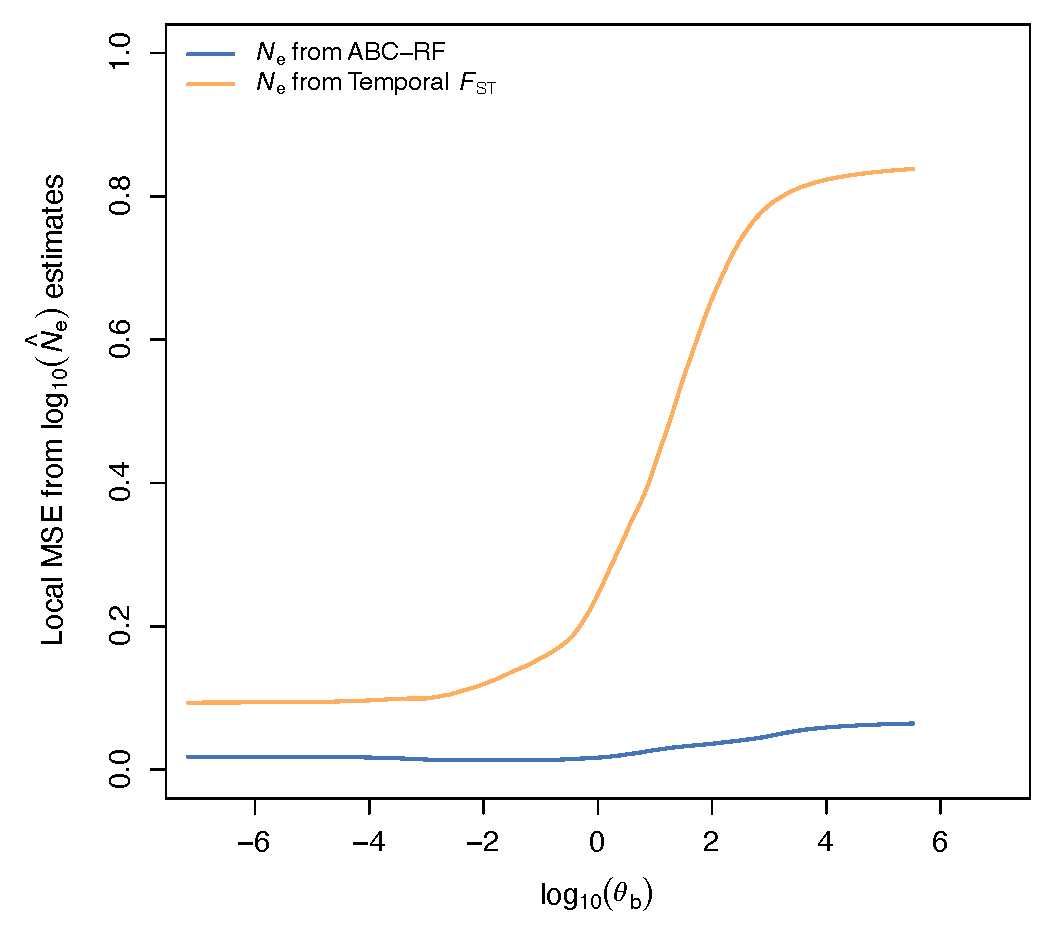
\includegraphics[width=0.50\textwidth]{Figures/main_text/Figure3_abcrfNE_fstNE_local_mse.pdf}
%DIFDELCMD <   %%%
\DIFdelendFL \DIFaddbeginFL 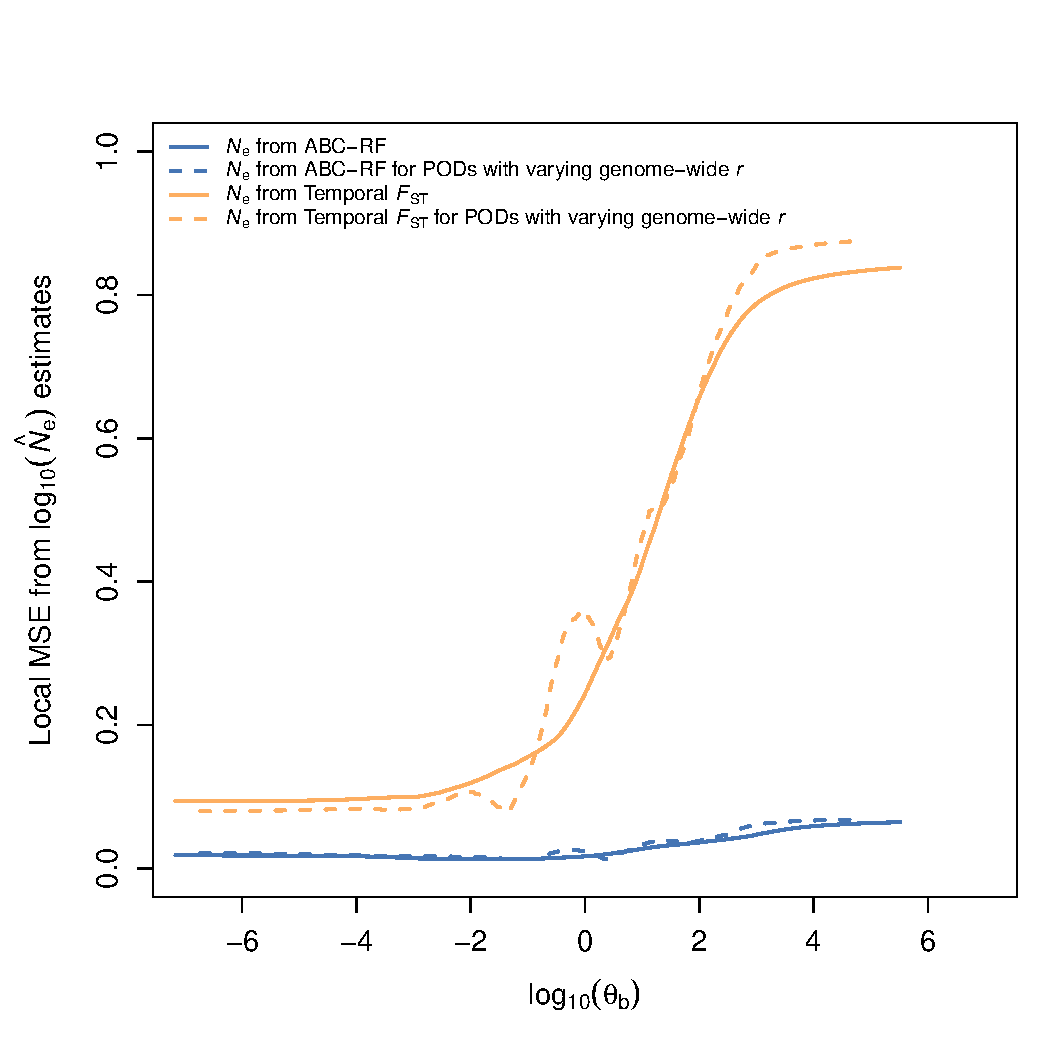
\includegraphics[width=0.50\textwidth]{Figures/Figure3_abcrfNE_fstNE_local_mse_recomb.pdf}
 \DIFaddendFL \small\caption{\textbf{Local MSE of $N_{\mathrm{e}}$ estimates as a function of $\theta_{\mathrm{b}}$.} The lines corresponds to the MSE on $N_{\mathrm{e}}$ estimates from ABC-RF and from temporal $F_{\mathrm{ST}}$. \DIFaddbeginFL \DIFaddFL{Dashed lines correspond to local MSE estimated from pseudo-observed data (POD) with heterogeneous recombination rates along the genome.}\DIFaddendFL }
 \label{fig:local_mse_nes}
\end{figure}

\subsection*{Analysis of temporal genomic data of feral populations of \textit{Apis mellifera}}

\DIFaddbegin \DIFadd{The projection of each population target data point (in black) into the cloud of the training data points (in grey) in the PCA plots revealed that each population model could capture some dimension of the observed genetic diversity (Figures~S8-S14). However, some PCs showed the observed data point outside the simulated data cloud of points, indicating some model inadequacies, possibly because we did not include gene flow or admixture in our simulations. }\DIFaddend For the analysis of feral \textit{A.\DIFaddbegin \DIFadd{\ }\DIFaddend mellifera} populations, we first grew independent RF for each parameter in each population. \DIFdelbegin \DIFdel{All populations had the same }\DIFdelend \DIFaddbegin \DIFadd{Despite the differences in time intervals between samples, all populations had a similar }\DIFaddend performance of the ABC-RF estimator for $N_{\mathrm{e}}$, as they showed similar values of MSE and $R^2$ (Figure \DIFdelbegin \DIFdel{S8}\DIFdelend \DIFaddbegin \DIFadd{S15}\DIFaddend ). For $N$, trained RF for Humboldt, Stebbins and Placerita performed similarly well, \DIFdelbegin \DIFdel{and they had }\DIFdelend \DIFaddbegin \DIFadd{with }\DIFaddend the lowest MSE and higher $R^2$ (Figure \DIFdelbegin \DIFdel{S7}\DIFdelend \DIFaddbegin \DIFadd{S16}\DIFaddend ). For $\theta_\mathrm{b}$, Riverside had trained RF with the worst performance (Figure \DIFdelbegin \DIFdel{S6}\DIFdelend \DIFaddbegin \DIFadd{S17}\DIFaddend ). Overall, both MSE and $R^2$ obtained with OOB estimates from simulated data for \textit{\DIFdelbegin \DIFdel{Apis }\DIFdelend \DIFaddbegin \DIFadd{A.\ }\DIFaddend mellifera} dataset were comparable to these parameters obtained with OOB estimates for the simulated data \DIFdelbegin \DIFdel{for }\DIFdelend \DIFaddbegin \DIFadd{in }\DIFaddend the evaluation of the method. 

Trained \DIFdelbegin \DIFdel{RF }\DIFdelend \DIFaddbegin \DIFadd{RFs }\DIFaddend for $N$ and $N_{\mathrm{e}}$ were able to predict these parameters in all populations, as the inference of the mean posterior value and the posterior distribution differentiated from the mean prior value and distribution (Figure~\ref{fig:postBees_jointdemosel} b and c). For $N$, posterior distribution were wider than for $N_{\mathrm{e}}$. Trained RF for $\theta_{\mathrm{b}}$, for all populations had a similar posterior mean, except for the Avalon population that had a peak at a lower value (Figure~\ref{fig:postBees_jointdemosel} a). \DIFdelbegin \DIFdel{But}\DIFdelend \DIFaddbegin \DIFadd{However}\DIFaddend , the posterior distributions were wider and \DIFdelbegin \DIFdel{they }\DIFdelend followed the prior distribution, making it difficult to \DIFdelbegin \DIFdel{accurately }\DIFdelend predict the posterior mean and variance in all populations \DIFaddbegin \DIFadd{accurately}\DIFaddend . It is possible to see together with the posterior mean estimates that the ABC-RF estimates for $\theta_{\mathrm{b}}$ were concentrated in lower values (Table \DIFdelbegin \DIFdel{S2}\DIFdelend \DIFaddbegin \DIFadd{S3}\DIFaddend ) in all populations. $N_{\mathrm{e}}$ were also lower, and $N_{\mathrm{e}}$ and $N$ were similar. For the results of OOB estimates of other model parameters and latent variables \DIFdelbegin \DIFdel{, and for }\DIFdelend \DIFaddbegin \DIFadd{and }\DIFaddend posterior estimates for these parameters\DIFdelbegin \DIFdel{see S3 }\DIFdelend \DIFaddbegin \DIFadd{, see section S2 }\DIFaddend Supplementary Results.


% Posterior estimates of joint demography and selection inference for feral bee populations
\begin{figure}[htb]
 \centering
 \DIFdelbeginFL %DIFDELCMD < \includegraphics[width=1\textwidth]{Figures/main_text/Figure4_weighted_densityPlots_jointDemoSel_feralbees.pdf}
%DIFDELCMD <   %%%
\DIFdelendFL \DIFaddbeginFL \includegraphics[width=1\textwidth]{Figures/Figure4_weighted_densityPlots_jointDemoSel_feralbees.pdf}
 \DIFaddendFL \small\caption{\DIFdelbeginFL \textbf{\DIFdelFL{Joint inference of demography and selection for feral }\textit{\DIFdelFL{A. mellifera}} %DIFAUXCMD
\DIFdelFL{populations.}} %DIFAUXCMD
\DIFdelendFL \DIFaddbeginFL \textbf{\DIFaddFL{Inference of demography and selection for feral }\textit{\DIFaddFL{A. mellifera}} \DIFaddFL{populations.}} \DIFaddendFL (a) the \DIFaddbeginFL \DIFaddFL{scale mutation rate of selected mutations $\theta_{\mathrm{b}}$, (b) the }\DIFaddendFL population census size $N$, (\DIFdelbeginFL \DIFdelFL{b}\DIFdelendFL \DIFaddbeginFL \DIFaddFL{c}\DIFaddendFL ) the effective population size $N_{\mathrm{e}}$\DIFdelbeginFL \DIFdelFL{(c) the scale mutation rate of selected mutations $\theta_{\mathrm{b}}$}\DIFdelendFL . Dashed and filled lines \DIFdelbeginFL \DIFdelFL{corresponds }\DIFdelendFL \DIFaddbeginFL \DIFaddFL{correspond }\DIFaddendFL to the prior and posterior distributions, respectively\DIFaddbeginFL \DIFaddFL{. See Table S3, Supplementary Results for mean and 95\% credibility intervals.}\DIFaddendFL }
 \label{fig:postBees_jointdemosel}
\end{figure}

\section*{Discussion}

\subsection*{Separating demography from drift, and the inference of $\theta_{\mathrm{b}}$}

With temporal population genomics data, we can see the evolution in ``action'' as opposed to single time-point population genomics data \citep{Feder:2021bt}. Consequently, temporal data have more information about the ongoing process, \DIFdelbegin \DIFdel{which make them better for the understanding of }\DIFdelend \DIFaddbegin \DIFadd{making them interesting for understanding }\DIFaddend the \DIFdelbegin \DIFdel{complex }\DIFdelend \DIFaddbegin \DIFadd{short-term effects of the }\DIFaddend interaction between demography and selection \citep{Buffalo:2019ab, Dehasque:2020ku, Williams:2020gk}. When samples from more than \DIFdelbegin \DIFdel{two time }\DIFdelend \DIFaddbegin \DIFadd{two-time }\DIFaddend points are available, \DIFdelbegin \DIFdel{the footprints }\DIFdelend \DIFaddbegin \DIFadd{correlations among allele frequency changes allow to separate the effects }\DIFaddend of drift and selection \DIFdelbegin \DIFdel{in allele frequencies changes can be separated \mbox{%DIFAUXCMD
\citep[e.g.,][]{Buffalo:2020hq,Feder:2014fe}}\hspace{0pt}%DIFAUXCMD
}\DIFdelend \DIFaddbegin \DIFadd{\mbox{%DIFAUXCMD
\citep[e.g.,][]{Buffalo:2020hq, Feder:2014fe}}\hspace{0pt}%DIFAUXCMD
}\DIFaddend . Our results showed that two samples collected \DIFdelbegin \DIFdel{in }\DIFdelend \DIFaddbegin \DIFadd{at }\DIFaddend different time points \DIFdelbegin \DIFdel{were }\DIFdelend \DIFaddbegin \DIFadd{are }\DIFaddend sufficient for the inference of the genome-wide footprint of adaptive evolution and to separate the demography (population census size $N$) from drift (effective population size $N_{\mathrm{e}}$). 

It is important to stress that $N_{\mathrm{e}}$, \DIFaddbegin \DIFadd{calculated }\DIFaddend as a latent variable, captures the feedback dynamics between drift and linked selection. Selection, either positive or negative, causes a deviation of $N_\mathrm{e}$ from $N$. The impact of selection on the genome can extend far from the target of selection since individuals that carry beneficial mutations have more chance to reproduce, \DIFaddbegin \DIFadd{and }\DIFaddend their beneficial mutations are more likely to be in the next-generation offspring \citep{Walsh:2018tv}. In this complex dynamic, with many loci under selection which creates a dynamic that cannot be easily described \DIFaddbegin \DIFadd{analytically}\DIFaddend , latent variables \DIFdelbegin \DIFdel{actually summarized the by product }\DIFdelend \DIFaddbegin \DIFadd{obtained from simulations can summarize the by-product }\DIFaddend of drift and selection interactions. With our approach, $\hat N_\mathrm{e}$ quantifies the drift due \DIFdelbegin \DIFdel{both }\DIFdelend to demographic and selection \DIFdelbegin \DIFdel{dynamics}\DIFdelend \DIFaddbegin \DIFadd{processes, unaffected by the bias of outlier loci}\DIFaddend .

This genome-wide reduction in $N_{\mathrm{e}}$ is not captured when loci are assumed to evolve independently \DIFdelbegin \DIFdel{\mbox{%DIFAUXCMD
\citep[as in][for example]{Sheehan:2016caa}}\hspace{0pt}%DIFAUXCMD
}\DIFdelend \DIFaddbegin \DIFadd{\mbox{%DIFAUXCMD
\citep[as in][for example]{Sheehan:2016caa, Laval:2019jo}}\hspace{0pt}%DIFAUXCMD
}\DIFaddend . In contrast, the complexity of linked selection and the genome-wide effect of selection are taken into account \DIFdelbegin \DIFdel{by using individual based simulations with }\DIFdelend \DIFaddbegin \DIFadd{using individual-based simulations with the }\DIFaddend whole genome in an ABC approach. 

Estimates of genetic load or other genome-wide parameters about selection are obtained when annotated genomic data is available \DIFdelbegin \DIFdel{, \mbox{%DIFAUXCMD
\citep{Henn:2015ce}}\hspace{0pt}%DIFAUXCMD
}\DIFdelend \DIFaddbegin \DIFadd{\mbox{%DIFAUXCMD
\citep{Henn:2015ce}}\hspace{0pt}%DIFAUXCMD
, }\DIFaddend or by conducting experiments on crossing populations \DIFdelbegin \DIFdel{(for the genetic load \mbox{%DIFAUXCMD
\citet{Plough:2016gw}}\hspace{0pt}%DIFAUXCMD
)}\DIFdelend \DIFaddbegin \DIFadd{\mbox{%DIFAUXCMD
\citep[for the genetic load;][]{Plough:2016gw}}\hspace{0pt}%DIFAUXCMD
}\DIFaddend . However, we \DIFdelbegin \DIFdel{were able to obtain }\DIFdelend \DIFaddbegin \DIFadd{obtained }\DIFaddend estimates of selection parameters only \DIFdelbegin \DIFdel{with }\DIFdelend \DIFaddbegin \DIFadd{using }\DIFaddend polymorphism data. \DIFdelbegin \DIFdel{A similar approach was used by \mbox{%DIFAUXCMD
\citet{Laval:2019jo} }\hspace{0pt}%DIFAUXCMD
to estimate the number of selective sweeps affecting the human genome in the past 10,000 years. But they did not consider the feedback dynamics of selection and demography. }\DIFdelend Differently, \citet{Buffalo:2020hq} measured the genome-wide signature of selection by estimating the covariance of allele frequencies at consecutive time points. \DIFdelbegin \DIFdel{This }\DIFdelend \DIFaddbegin \DIFadd{The allele frequency covariance matrix }\DIFaddend allowed the quantification of the genome-wide contribution of selection to the observed allele frequency changes, even when selection involved many loci of small effect. In this work, we estimated the population scale mutation rate of beneficial mutations $\theta_{\mathrm{b}}$, which informs about the diversity of beneficial mutations that existed in the population between the two time points \DIFdelbegin \DIFdel{, }\DIFdelend and the potential speed of adaptation at the genome level \citep{Hermisson:2017hw}. These estimates reflect the potential number of beneficial mutations \DIFdelbegin \DIFdel{present between the two time points regardless }\DIFdelend \DIFaddbegin \DIFadd{between the two-time points regardless of }\DIFaddend their impact as determined by their selection coefficients.

The variable importance plot of each parameter shows us the global importance of each summary \DIFdelbegin \DIFdel{statistics }\DIFdelend \DIFaddbegin \DIFadd{statistic }\DIFaddend in the trained Random Forests. For $N_{\mathrm{e}}$, $N$, and $\theta_{\mathrm{b}}$ summary statistics calculated from the distribution of locus-specific summary statistics -skewness, kurtosis, mean, variance, 5\% and 95\% quantiles were more frequently used. Summary statistics derived from the distribution of locus-specific calculated from all segregating loci in the genome inform about the heterogeneity that selection and drift produce genome-wide. For example, a \textit{de novo} a beneficial mutation entered the simulation and was selected\DIFdelbegin \DIFdel{, }\DIFdelend \DIFaddbegin \DIFadd{; }\DIFaddend it left a signal of lower diversity around the region it was located. The genome, after selection, contained spots where diversity was high and where it was low, and this heterogeneity was captured by the distribution of locus-specific $H_{\mathrm{E}}$, more specifically\DIFaddbegin \DIFadd{, }\DIFaddend the lower tail of the distribution where the \DIFdelbegin \DIFdel{values of diversity }\DIFdelend \DIFaddbegin \DIFadd{diversity values of the statistic }\DIFaddend were lower. The \DIFdelbegin \DIFdel{use of the }\DIFdelend covariance matrix of allele frequencies through \DIFdelbegin \DIFdel{\mbox{%DIFAUXCMD
\citet{Buffalo:2020hq} }\hspace{0pt}%DIFAUXCMD
can be considered }\DIFdelend \DIFaddbegin \DIFadd{time \mbox{%DIFAUXCMD
\citep{Buffalo:2020hq} }\hspace{0pt}%DIFAUXCMD
can be used }\DIFaddend as a summary statistic \DIFdelbegin \DIFdel{for the the genome-wide heterogeneity that }\DIFdelend \DIFaddbegin \DIFadd{to capture additional information about the }\DIFaddend selection and drift \DIFdelbegin \DIFdel{left on the genome. It would be interesting to include }\DIFdelend \DIFaddbegin \DIFadd{when more than two temporal samples are available. Including }\DIFaddend this matrix as summary statistics for further development of the method \DIFaddbegin \DIFadd{would be interesting}\DIFaddend .

\subsection*{Comparison with $F_{\mathrm{ST}}$ method to estimate $N_\mathrm{e}$}

We compared the $N_{\mathrm{e}}$ obtained with ABC-RF framework to the $N_{\mathrm{e}}$ obtained with $F_{\mathrm{ST}}$ estimator \DIFdelbegin \DIFdel{\mbox{%DIFAUXCMD
\citep{Skoglund:2014ci, Frachon:2017fw}}\hspace{0pt}%DIFAUXCMD
}\DIFdelend \DIFaddbegin \DIFadd{\mbox{%DIFAUXCMD
\citep{Frachon:2017fw}}\hspace{0pt}%DIFAUXCMD
}\DIFaddend . Overall, the $F_{\mathrm{ST}}$-based $N_{\mathrm{e}}$ estimator performed poorly compared to the \DIFdelbegin \DIFdel{ABC-RF -based }\DIFdelend \DIFaddbegin \DIFadd{ABC-RF-based }\DIFaddend estimator. The lower performance \DIFdelbegin \DIFdel{were }\DIFdelend \DIFaddbegin \DIFadd{was }\DIFaddend caused by $N_{\mathrm{e}}$ values that were underestimated when beneficial mutations were more frequent (higher $\theta_{\mathrm{b}}$). Consequently, the $N_{\mathrm{e}}$ estimates from the temporal $F_{\mathrm{ST}}$ were strongly affected by selection. \DIFdelbegin \DIFdel{When }\DIFdelend \DIFaddbegin \DIFadd{Both estimators performed similarly when the }\DIFaddend selection was infrequent or rare, \DIFdelbegin \DIFdel{both estimators performed similarly well, but with }\DIFdelend \DIFaddbegin \DIFadd{but }\DIFaddend the ABC-RF estimator \DIFdelbegin \DIFdel{with lower MSE }\DIFdelend \DIFaddbegin \DIFadd{had lower MSE than the $F_{\mathrm{ST}}$ one}\DIFaddend . Positive selection can increase the variance of allele frequency between samples taken \DIFdelbegin \DIFdel{in }\DIFdelend \DIFaddbegin \DIFadd{at }\DIFaddend different time points. When selection is infrequent or rare, drift determines most \DIFdelbegin \DIFdel{of }\DIFdelend allele frequency changes between samples\DIFdelbegin \DIFdel{; but }\DIFdelend \DIFaddbegin \DIFadd{. Still, }\DIFaddend when selection is pervasive, selection dominates, which \DIFdelbegin \DIFdel{cause }\DIFdelend \DIFaddbegin \DIFadd{causes }\DIFaddend dramatic and rapid changes in allele frequency, increasing the variance between samples. $N_{\mathrm{e}}$ estimator based on the $F_{\mathrm{ST}}$ depends on the differences in allele frequencies between samples\DIFdelbegin \DIFdel{, consequently}\DIFdelend \DIFaddbegin \DIFadd{; consequently, }\DIFaddend it is naturally biased by strong and frequent selection. We can assume that the $N_{\mathrm{e}}$ estimator from ABC-RF was insensitive to the amount of selection since we trained the ABC-RF with $N_{\mathrm{e}}$ values from the simulation. In our simulations, $N_{\mathrm{e}}$ was a latent variable that captured the deviation that selection imposed on the number of individuals able to reproduce (selected for); \DIFdelbegin \DIFdel{it was not a biased by unaccounted factors }\DIFdelend \DIFaddbegin \DIFadd{unaccounted factors did not bias it}\DIFaddend . 

The amount of selection for \DIFdelbegin \DIFdel{$\theta_{\mathrm{b}}\sim O(1)$ }\DIFdelend \DIFaddbegin \DIFadd{$\theta_{\mathrm{b}} > 1$ }\DIFaddend could be unrealistic in some organisms, but plausible in virus \citep{Feder:2014fe} and many arthropod species, with large $N_{\mathrm{e}}$, which have larger population sizes \DIFdelbegin \DIFdel{(except in eusocial insects that have vertebrate-like population sizes \mbox{%DIFAUXCMD
\citet{Romiguier:2014dh}}\hspace{0pt}%DIFAUXCMD
). In larger populations sizes selection acts also }\DIFdelend \DIFaddbegin \DIFadd{\mbox{%DIFAUXCMD
\citep[except in eusocial insects that have vertebrate-like population sizes;][]{Romiguier:2014dh}}\hspace{0pt}%DIFAUXCMD
. The selection also acts }\DIFaddend on weaker and milder beneficial mutations \DIFaddbegin \DIFadd{in larger populations}\DIFaddend . In those organisms, it might be unreasonable to assume mutation-drift equilibrium given the pervasive role of selection. Consequently, \DIFdelbegin \DIFdel{any attempt }\DIFdelend \DIFaddbegin \DIFadd{attempts }\DIFaddend to estimate demography parameters as $N_{\mathrm{e}}$ without properly accounting for the pervasive role of selection could be biased.

\subsection*{Analysis of temporal genomic data of feral populations of \textit{Apis mellifera}}

Overall, the performance of the ABC-RF for selection and demography inference was similar across populations despite the differences in sample size and age. For $\theta_{\mathrm{b}}$, Avalon and Humboldt populations had posterior probability distributions \DIFdelbegin \DIFdel{very }\DIFdelend similar to the prior, indicating that the analysis provides no additional information on this parameter. These two \DIFdelbegin \DIFdel{population }\DIFdelend \DIFaddbegin \DIFadd{populations }\DIFaddend also present low effective population size estimates, \DIFdelbegin \DIFdel{which can reduce the signal of selection }\DIFdelend \DIFaddbegin \DIFadd{reducing the selection signal}\DIFaddend . For the rest of the populations, the posterior probability distribution of $\theta_{\mathrm{b}}$ is tilted toward the higher values but without a clear peak differentiating the distribution from the prior. Still, lower $\theta_{\mathrm{b}}$ values could be excluded. \DIFdelbegin \DIFdel{This favours an interpretation in which }\DIFdelend \DIFaddbegin \DIFadd{It favors the interpretation that }\DIFaddend selection was acting during the study period \DIFdelbegin \DIFdel{but }\DIFdelend without providing a precise \DIFdelbegin \DIFdel{estimate of the parameter . The information about the }\DIFdelend \DIFaddbegin \DIFadd{parameter estimate. The }\DIFaddend presence of selection in these analyses comes mainly from the heterogeneity of the polymorphism along the genome\DIFdelbegin \DIFdel{, thus}\DIFdelend \DIFaddbegin \DIFadd{. Thus}\DIFaddend , for a thorough interpretation of the results, it is important to discuss other processes that have not been \DIFdelbegin \DIFdel{modelled but that }\DIFdelend \DIFaddbegin \DIFadd{modeled but }\DIFaddend could affect this signal.
The studied bee populations in California show a mixture of Eastern and Western European ancestry, with some populations presenting African ancestry in the most modern samples \citet{Cridland:2018fx}. Different levels of African admixture along the genome could create some heterogeneity and affect the inference. However, \DIFaddbegin \DIFadd{in }\DIFaddend Placerita and Riverside, the populations with higher African ancestry \DIFdelbegin \DIFdel{at present, }\DIFdelend present similar estimates of $\theta_{\mathrm{b}}$ that populations with little or no African admixture. \DIFdelbegin \DIFdel{Also, Humboldt population changes from having }\DIFdelend \DIFaddbegin \DIFadd{The Humboldt population changed from }\DIFaddend predominately Western European \DIFdelbegin \DIFdel{ancestry to having predominately }\DIFdelend \DIFaddbegin \DIFadd{to }\DIFaddend Eastern European ancestry, \DIFdelbegin \DIFdel{which means }\DIFdelend \DIFaddbegin \DIFadd{meaning }\DIFaddend that there was substantial gene flow into the population. These results suggest that admixture does not dramatically affect the inference of selection but also highlights the importance of incorporating admixture in \DIFaddbegin \DIFadd{the }\DIFaddend future development of the approach. \DIFaddbegin \DIFadd{Other processes, such as recombination and mutation rate, might be heterogeneous along the genome. Our analysis of simulations with heterogeneous recombination rate suggest that the approach is robust to those. However, more complex models also seem necessary to fully capture the observed genetic diversity (see Figures~S7-S13, section S2 Supplementary Results). Including additional factors (admixture, heterogeneity of recombination and mutation rate, and other forms of selection) could be key to obtaining models that fit the data better. Further developments of this approach should take them into account.
}\DIFaddend 

%NOTE ABOUT VARROA, I DO NOT SEE WHY DO YOU MENTION IT. ADAPTATION COULD BE TO ANY OTHER THING AND MULTIPLE THIGS. HAS VARROA ARRIVED IN THE TIME INTERVAL STUDIED? OTHERWISE, I DO NOT SEE ANY REASON TO MENTION IT. REGARDING THE INFLUENCE OF AFRICAN ADMIXTURE FOR THE RESISTANCE TO VARROA, OUR METHOD IS NOT ADAPTED TO SUCH FORM OF SELECTION (ADAPTIVE ADMIXTURE/INTROGRESSION) SO I WOULD NOT GET INTO THAT.

% The interpretation is that little or no selection occurred between the first and the second time sample. For the Humboldt population, low values of $\N{\mathrm{e}}$ might also reflects the low genetic diversity of this population, either because of the occurrence of a bottleneck determined by the arrival of \textit{Varroa} or by an adaptation to this mite species. \textit{Varroa} is a mite group known for causing significant infestations in bee colonies, to the point of the entire elimination of the nest. Bees from the African lineage or bees that have some African ancestry (Africanized bees that acquired the African ancestry through introgression) are more tolerant to \textit{Varroa} infestations. The arrival of \textit{Varroa} in California caused a severe population reduction, especially in northern populations, because these populations present no African ancestry. The African ancestry in the southern population (up to 42\%), however, might have decreased the susceptibility to \textit{Varroa} infestations \citep{Calfee:2020hd}, allowing these populations thrive and keep the same population size. The Africanization of the southern also increased the adaptive potential of these populations, which could see in the more positive values of $\theta_{\mathrm{b}}$. The distributions of $\theta_{\mathrm{b}}$ estimated by our model in the southern populations might also reflect the genomic heterogeneity's determined by admixture, not by selection alone since admixture can create heterogeneity in the genome. To separate adaptation from admixture, we should jointly model these effects by simulating selection in admixed populations.

Our ABC-RF approach estimated $N_\mathrm{e}$ with the same order of magnitude of other $N_\mathrm{e}$ estimates obtained for hymenopterans \citep{Zayed:2004kg}.
%Lower values of $N_\mathrm{e}$ and $\theta_{\mathrm{b}}$ might be a consequence of the the impact of caused by \textit{Varroa} infestation.
Lower values of $N_\mathrm{e}$ might reflect the presence of admixture, either African admixture or admixture that occurred with domesticated lineages facilitated by changes in beekeeping practices \DIFaddbegin \DIFadd{\mbox{%DIFAUXCMD
\citep{Cridland:2018fx}}\hspace{0pt}%DIFAUXCMD
}\DIFaddend . Northern populations, especially from Humboldt County, shared similarities with bees from reared colonies (with higher Eastern European ancestry). Southern populations, as shown by \citet{Cridland:2018fx}\DIFaddbegin \DIFadd{, }\DIFaddend showed a higher level of admixture with African lineages. Populations from the southernmost \DIFdelbegin \DIFdel{cites (from }\DIFdelend \DIFaddbegin \DIFadd{cities (}\DIFaddend Riverside County, Placerita, and Avalon, Los Angeles \DIFdelbegin \DIFdel{county}\DIFdelend \DIFaddbegin \DIFadd{County}\DIFaddend ) showed higher genetic diversity \DIFdelbegin \DIFdel{, but they }\DIFdelend \DIFaddbegin \DIFadd{than the others but }\DIFaddend did not show the highest values of $N_\mathrm{e}$. On the other hand, the population of Stanislaus County had the highest value of $N_\mathrm{e}$, possibly because it had lower levels of admixture with domesticated lineages compared to the population from Riverside, Placerita, Avalon, and Los Angeles \DIFdelbegin \DIFdel{county}\DIFdelend \DIFaddbegin \DIFadd{counties}\DIFaddend .

We observed that $N_\mathrm{e}$ and $N$ had similar estimates. We were aware that our simulation model did not account for key characteristics of eusocial insect reproductive biology: the monopolization of reproduction by the queen and the division of labor. In \DIFdelbegin \DIFdel{Honey }\DIFdelend \DIFaddbegin \DIFadd{honey }\DIFaddend bees, a queen mates with more than one male (a process called polyandry)\DIFdelbegin \DIFdel{\mbox{%DIFAUXCMD
\citep{Estoup:jj}}\hspace{0pt}%DIFAUXCMD
}\DIFdelend , which leads to a biased breeding sex ratio \DIFaddbegin \DIFadd{\mbox{%DIFAUXCMD
\citep{Estoup:jj}}\hspace{0pt}%DIFAUXCMD
}\DIFaddend . Assuming that only queens can reproduce in the colony, polyandry increases the variance in the number of parents \DIFdelbegin \DIFdel{that contribute }\DIFdelend \DIFaddbegin \DIFadd{contributing }\DIFaddend to the offspring gene pool, which leads to a decrease in the $N_\mathrm{e}$ compared \DIFdelbegin \DIFdel{respect }\DIFdelend to $N$ \citep{Nomura:2012bp}. In our simulations, we only simulated \DIFdelbegin \DIFdel{monogamous mating, therefore}\DIFdelend \DIFaddbegin \DIFadd{panmictic random mating. Therefore}\DIFaddend , the difference between estimates of $N_\mathrm{e}$ and $N$ only reflects the \DIFdelbegin \DIFdel{action of selection }\DIFdelend \DIFaddbegin \DIFadd{selection action}\DIFaddend . Therefore $N$ must be interpreted with caution as it is probably reflecting more the total number of female breeders per generation rather than the size of the population. Individual-based forward simulators \DIFaddbegin \DIFadd{such }\DIFaddend as SLiM allows setting different mating schemes. It is possible to simulate the haplodiploidy, the cast system, diocy\DIFaddbegin \DIFadd{, }\DIFaddend and sex ratio found in honey bees. These \DIFdelbegin \DIFdel{modifications in the simulation could potentially }\DIFdelend \DIFaddbegin \DIFadd{simulation modifications could }\DIFaddend allow us to estimate $N$ and other parameters that could \DIFdelbegin \DIFdel{reflect better the biology of the speciesbut it }\DIFdelend \DIFaddbegin \DIFadd{better reflect the species' biology, but that }\DIFaddend was not the focus of this work.

%measured the effective population size ($N_\mathrm{e}$). To model the difference between $N_\mathrm{e}$ and $N$, more generally, it is necessary to simulate the haplodiploidy and the cast system. To capture the difference in sex ratio found in honey bees, it is also necessary to model dioecy. These modifications would allow us to estimate $N$ that captures the number of colonies in the population, not reproducing individuals. We could even increase the model complexity by including key and specific components of the reproductive biology of honey bees. In Honey bees, a queen mates with more than one male (a process called polyandry) \citep{Estoup:jj}, which leads to a biased breeding sex ratio. Assuming that only queens can reproduce in the colony, polyandry increases the variance in the number of parents that contribute to the offspring gene pool, which leads to a decrease in the $N_\mathrm{e}$ compared to a monogamous mating system \citep{Nomura:2012bp}. In our simulations, we only simulated monogamous mating; the inclusion of polyandry could, in theory, increase the estimate of $N$.
%Honey bees also have a polymorphism in the complementary sex determination (CDS) genes. In bees, sex depends on the ploidy: females (queens or workers) are diploid, and they are the product of sexual reproduction; males are haploid, produced by the queen (or worker in some cases) by the development of unfertilized eggs. In addition to ploidy, sex also depends on the CDS genes: a heterozygote for the CDS gene develops as female; a homozygote as male. In honey bees, the variability in the complementary sex determination (CDS) genes also reduce the $N_\mathrm{e}$ \citep{Zayed:2004kg}. The CDS effect on $N_\mathrm{e}$ is greater when combined with polyandry \citep{Zayed:2004kg}. Individual-based forward simulators as SLiM allows setting different mating schemes as complex as present in honey bees. Thus, there is a potential to include the modeling of polyandry or other mating systems in the proposed inference framework.

One possible explanation for the similarities between $N_\mathrm{e}$ and $N$ estimates, thus, relies on cast specialization and concentration of reproduction to one of few females in the colony. These came to a cost of reduced $N_{\mathrm{e}}$, which reduces the efficacy of selection (either positive or negative). Bees are the few insect groups that show very small $N_{\mathrm{e}}$ potentially linked with the evolution of eusociality \citep{Romiguier:2014dh}. Knowing that lower $N_{\mathrm{e}}$ reduces the effectiveness of selection, it is plausible to think that lower $N_\mathrm{e}$ is restricting the effects of mutation affecting fitness to stronger beneficial mutations. Since these mutations are less frequent than weak or mild mutations, their effects on $N_\mathrm{e}$ were small, which explains why $N_\mathrm{e}$ and $N$ had values in the same range. Low $N_\mathrm{e}$ and low $\theta_{\mathrm{b}}$ pointed to a biological system limited where adaptation is limited by the influx of adaptive mutations \citep{Rousselle:2020ct}.

Our ABC-RF framework also estimated the per-site mutation rate per generation $\mu$ (Supplementary Results, S18). \DIFdelbegin \DIFdel{For all populations, the }\DIFdelend \DIFaddbegin \DIFadd{The }\DIFaddend mean posterior $\mu$ \DIFaddbegin \DIFadd{for all populations }\DIFaddend exceeds the mean \DIFaddbegin \DIFadd{prior }\DIFaddend $\mu$\DIFdelbegin \DIFdel{of the species}\DIFdelend . The higher estimated values we obtained might \DIFdelbegin \DIFdel{reflect the }\DIFdelend \DIFaddbegin \DIFadd{be due to the higher true mutation rate but also reflect }\DIFaddend recent admixture events between these populations. \DIFdelbegin \DIFdel{We did not model gene flow and admixture. }\DIFdelend Modeling admixture could help us correctly separate the effects of selection and drift since the introgression of African genes might have biased some estimates of selection parameters.

\subsection*{Perspectives and Limitations}

Our model is \DIFdelbegin \DIFdel{very simplistic}\DIFdelend \DIFaddbegin \DIFadd{relatively simple}\DIFaddend , as it only considered the impact of beneficial mutations, neglecting the effect of background selection and standing variation. Background selection can mimic directional selection because they cause a similar pattern of diversity reduction around the target of selection \DIFdelbegin \DIFdel{. However, it was recently shown that background selection only mimics the classical sweepin simplistic models, where the deleterious mutation is localized in a specific region }\DIFdelend \DIFaddbegin \DIFadd{\mbox{%DIFAUXCMD
\citep{Stephan:2010} }\hspace{0pt}%DIFAUXCMD
has been discussed for a long time. Much less has been discussed about the patterns of background selection on temporal data and their differences with selective sweeps. \mbox{%DIFAUXCMD
\citet{Cvijovic:2018} }\hspace{0pt}%DIFAUXCMD
showed that neutral alleles linked to less deleterious backgrounds could quickly rise to high frequencies due to purifying selection, which could mimic the temporal signal of a selective sweep. However, if background selection is not localized to specific regions }\DIFaddend of the genome\DIFdelbegin \DIFdel{\mbox{%DIFAUXCMD
\citep{Schrider:2020hka}}\hspace{0pt}%DIFAUXCMD
. For more realistic scenarios, where the concentration of deleterious mutations varies across the genome, background selection does not behave as a classical hard sweep}\DIFdelend \DIFaddbegin \DIFadd{, the signal of selective sweeps will be distinct from the effects of background selection \mbox{%DIFAUXCMD
\citep{Schrider:2020hka}}\hspace{0pt}%DIFAUXCMD
}\DIFaddend . In an attempt to jointly accommodate the effect of demography and selection on the inference of $N_{\mathrm{e}}$, \citet{Johri:2020ee} modeled the effect of background selection and developed an ABC-based approach that jointly estimated the distribution of fitness effects and $N_{\mathrm{e}}$. In their simulations, they modeled deleterious mutations and the classical hard sweep with the inclusion of beneficial mutations. They showed an unbiased estimate of $N_{\mathrm{e}}$ regardless of \DIFdelbegin \DIFdel{the presence of }\DIFdelend positive and negative selection \DIFaddbegin \DIFadd{presence}\DIFaddend . Future developments should include a more realistic genomic architecture \DIFdelbegin \DIFdel{where both }\DIFdelend \DIFaddbegin \DIFadd{were }\DIFaddend negative and positive mutations can co-occur and explore different concentrations of deleterious mutations. In addition\DIFdelbegin \DIFdel{to that}\DIFdelend , further developments should explore \DIFdelbegin \DIFdel{not only }\DIFdelend scenarios of \textit{de novo} mutations \DIFdelbegin \DIFdel{, but }\DIFdelend \DIFaddbegin \DIFadd{and }\DIFaddend selection acting on standing variation. \DIFdelbegin \DIFdel{This can be easily }\DIFdelend \DIFaddbegin \DIFadd{It can be }\DIFaddend achieved with our pipeline and allows for a more general treatment of the selection of soft sweeps. The model can also be expanded to more complex demographic scenarios, including changes in population size and genetic exchange with external sources (migration). Including such admixtures will be key in the future development of this approach since it is also a source of heterogeneity in the genome and, thus, might influence the \DIFdelbegin \DIFdel{performance of the method}\DIFdelend \DIFaddbegin \DIFadd{method's performance}\DIFaddend . 

\section*{Conclusion}

We show that an ABC-RF -based approach \DIFdelbegin \DIFdel{is able to }\DIFdelend \DIFaddbegin \DIFadd{can }\DIFaddend jointly infer adaptive and demographic history from temporal population genomics data. This approach \DIFdelbegin \DIFdel{allows the quantification of }\DIFdelend \DIFaddbegin \DIFadd{quantifies }\DIFaddend the genome-wide footprint of selection expressed in the scaled mutation rate of beneficial mutations. The ABC-RF $N_{\mathrm{e}}$ is robust to varying degrees of strength of selection and frequency of beneficial mutations. Our ABC-RF -based approach can be applied to temporal population genomics datasets to gain insight \DIFdelbegin \DIFdel{about the }\DIFdelend \DIFaddbegin \DIFadd{into natural populations' }\DIFaddend adaptive and demographic history\DIFdelbegin \DIFdel{of natural populations.
}%DIFDELCMD < 

%DIFDELCMD < %%%
\DIFdelend \DIFaddbegin \DIFadd{.
}\DIFaddend \section*{Acknowledgements}

This project has received funding from the LabEx AGRO (convention ANR-10-LABX-0001-01), CEMEB (convention ANR-10-LABX-0004)\DIFaddbegin \DIFadd{, }\DIFaddend and NUMEV (convention ANR-10-LABX-20) through the AAP Inter-LabEx (ABCSelection). This project has received funding from the European Union's Horizon 2020 research and innovation \DIFdelbegin \DIFdel{programme }\DIFdelend \DIFaddbegin \DIFadd{program }\DIFaddend under the Marie Skłodowska-Curie grant agreement No 791695 (TimeAdapt). S. De Mita was funded by INRAE (\textit{Projet Innovant EFPA}). We are thankful for the Genotoul bioinformatics platform Toulouse Occitanie (Bioinfo Genotoul, https://doi.org/10.15454/1.5572369328961167E12), for the High-Performance Computing Center University of Montpellier (MESO@LR-Platform) and for the Ohio Super Computer Center (OSC \citet{OhioSupercomputerCenter1987}) for providing computing resources. The authors would like to \DIFdelbegin \DIFdel{thanks }\DIFdelend \DIFaddbegin \DIFadd{thank }\DIFaddend Julie Cridland for sharing the processed data \DIFdelbegin \DIFdel{, }\DIFdelend and Andrew P. Michel for providing suggestions to improve an early version of the manuscript. 

\bibliographystyle{apalike}
\bibliography{references}

\end{document}

% removed from the text (bioRxiv verstion):
% But, they used a prior human demographic model, which prevented the jointly inference of demography and selection on $N_\mathrm{e}$. As a consequence, they did not account the potential reduction of $N_\mathrm{e}$ by selection and its effect on the parameter estimation of sweep. 


%Several methods have been developed for the analysis of temporal data: for the estimation of the $N_{\mathrm{e}}$ \citep{Nei:1981vb, Beaumont:2003jv, Tallmon:2004jp, Anderson:2005jw}; and for the inference of selection parameters \citep[for a review,][]{Malaspinas:2012dv}. For $N_{\mathrm{e}}$ inference, loci are assumed to evolve neutrally \citep{Nei:1981vb, Anderson:2005jw} and without the effect of new mutations that may appear during the time interval between samples \citep[but see,][]{Beaumont:2003jv}. For selection, mutations were modeled as evolving independently, which neglects linked selection \citep{Feder:2014fe,Schraiber:2016ks, FerrerAdmetlla:2016jc, Goldringer:2004ei}, selection coefficients were limited to a range of mild to strong selection coefficients \citep{Malaspinas:2012dv,Feder:2014fe,Gompert:2015hs}, and, more importantly, interaction between drift and selection is ignored, because  $N_{\mathrm{e}}$ is either estimated first \citep{Foll:2014kv, Foll:2015ce,  Goldringer:2004ei, Rego:2019ba}, or it is treated as a nuisance parameter \citep[for example,][]{Malaspinas:2012dv, Feder:2014fe}. Consequently, these methods suffer from the same limitations discussed above. However, a notrable exception is the approach proposed by \citet{Buffalo:2019ab} which quantifies the effects of genome-wide linked selection during recent polygenic adaptation. [<- this paragraph seems redundant with] [Should we remove it entirelly?]

%(\url{https://github.com/vitorpavinato/Tracking-selection/}) (doi:10.5281/zenodo.4599736)[I just added this in the last minute, I am not sure if I cited correctly]

%[maybe remove as suggested by Stéphane]The problems with row-wise missing data were more dramatic here as the genome size used here was 2.5x higher than the one used for the model proof. Memory intense simulations were killed by SLiM in varying simulation times, consequently we had reference tables for each longitudinal pair with different numbers of rows. For example, the population pair from Humboldt Riverside site (15 generations between samples) had 13,930, and the pair from Humboldt site (49 generations) had 14,216 rows 

%or by measuring the genome-wide covariance of allele frequencies through time \citep{Buffalo:2019ab, Buffalo:2020hq} [I'm not sure of this last part, to be discussed!] 

%Another way to estimate $N_{\mathrm{e}}$ with temporal data is to use the standardized variance in allele frequencies \citep{Nei:1981vb, Pollak:1983vf}. This was the approach proposed by \citet{Goldringer:2004ei} in their genome scan for temporal data. This was also the approach used by \citet{Foll:2014kv, Foll:2015ce} in their ABC framework for the inference of selection coefficients $s$, however using a different $N_{\mathrm{e}}$ calculation \citep{Jorde:2007ej}. It was pointed out that $N_{\mathrm{e}}$ estimates from $F_{\mathrm{C}}$ \citep{Nei:1981vb} are upwardly biased when allele frequencies are close to zero or one \citep{Waples:1989tv}. \citet{Turner:2001dx} found that the bias might be associated with the complex interaction among population allele frequency, true effective size, sample size, and the number of generations between samples. \citet{Jorde:2007ej} found bias for the above-mentioned $N_{\mathrm{e}}$ estimates and proposed one that was less affected by small population sizes and skewed distribution of allele frequencies. Although \citet{Jorde:2007ej} is less biased than \citep{Nei:1981vb} $F_{\mathrm{C}}$, it has greater variance. Genetic differentiation based on $F_{\mathrm{ST}}$ have better statistical properties in terms of bias and variance than $F_{\mathrm{C}}$ (or either \citet{Jorde:2007ej}'s $F'$). Consequently, $N_{\mathrm{e}}$ from $F_{\mathrm{ST}}$ is less biased and responds better to the genetic drift \citep{Skoglund:2014ci} making it ideal for the comparison with our ABC-RF derived $N_{\mathrm{e}}$ estimates.
%[<- I do not see the point of this discussion here (from the start of this paragraph to this point). You did not present any result for Fc and related estimates. What it is relevant is that all those estimates assume a neutral model.] 

%We decided to simulate with no missing data, but our pipeline can handle the presence of missing data in empirical dataset. It is done by randomly imputing missing genotypes given the percentage of missing data in the dataset.

%In haplodiploid organisms, if each queen only mate with one drone from another colony (monogamy), the number of queens and drones are approximated by the number of nests in the population. The neutral effective population size can be then approximated by:
%\begin{gather*}
%\hat N_\mathrm{e} = \frac{9 N_\mathrm{f} N_\mathrm{m} }{2 N_\mathrm{f} + 4 N_\mathrm{m}} 
%\end{gather*}

%A second explanation for $N_\mathrm{e}$ and $N$ be in the same range relies on the past but recent events that took place in California. Some events in the past might have drastically reduced the $N_\mathrm{e}$ before or in between the the samples were taken. Because the time between samples were not enough for the population recovery for the perturbation, $N_\mathrm{e}$ reflects the drastic changes in diversity caused by changes in beekeeping practices, the introduction of Africanized bees, the introduction of \textit{Varroa}, and the potential local adaptation of some populations to \textit{Varroa} \citet{Cridland:2018fx}. 

%We can also include polyandry as a prior (as the number of males that a queen mate, for example), and estimate it with our ABC-RF framework. CDS can be modeled by including a loci that depending on the combination of alleles, determine the sex of the individual in addition to the haplodiploidy. Because SLiM is a flexible simulator, it would be straightforward to incorporate these modifications in future implementations. 
